% interactcadsample.tex
% v1.03 - April 2017

\documentclass[]{interact}

\usepackage{epstopdf}% To incorporate .eps illustrations using PDFLaTeX, etc.
\usepackage{subfigure}% Support for small, `sub' figures and tables
%\usepackage[nolists,tablesfirst]{endfloat}% To `separate' figures and tables from text if required

\usepackage{natbib}% Citation support using natbib.sty
\bibpunct[, ]{(}{)}{;}{a}{}{,}% Citation support using natbib.sty
\renewcommand\bibfont{\fontsize{10}{12}\selectfont}% Bibliography support using natbib.sty

\theoremstyle{plain}% Theorem-like structures provided by amsthm.sty
\newtheorem{theorem}{Theorem}[section]
\newtheorem{lemma}[theorem]{Lemma}
\newtheorem{corollary}[theorem]{Corollary}
\newtheorem{proposition}[theorem]{Proposition}

\theoremstyle{definition}
\newtheorem{definition}[theorem]{Definition}
\newtheorem{example}[theorem]{Example}

\theoremstyle{remark}
\newtheorem{remark}{Remark}
\newtheorem{notation}{Notation}

% see https://stackoverflow.com/a/47122900
  \usepackage{color}
  \usepackage{fancyvrb}
  \newcommand{\VerbBar}{|}
  \newcommand{\VERB}{\Verb[commandchars=\\\{\}]}
  \DefineVerbatimEnvironment{Highlighting}{Verbatim}{commandchars=\\\{\}}
  % Add ',fontsize=\small' for more characters per line
  \usepackage{framed}
  \definecolor{shadecolor}{RGB}{248,248,248}
  \newenvironment{Shaded}{\begin{snugshade}}{\end{snugshade}}
  \newcommand{\AlertTok}[1]{\textcolor[rgb]{0.94,0.16,0.16}{#1}}
  \newcommand{\AnnotationTok}[1]{\textcolor[rgb]{0.56,0.35,0.01}{\textbf{\textit{#1}}}}
  \newcommand{\AttributeTok}[1]{\textcolor[rgb]{0.77,0.63,0.00}{#1}}
  \newcommand{\BaseNTok}[1]{\textcolor[rgb]{0.00,0.00,0.81}{#1}}
  \newcommand{\BuiltInTok}[1]{#1}
  \newcommand{\CharTok}[1]{\textcolor[rgb]{0.31,0.60,0.02}{#1}}
  \newcommand{\CommentTok}[1]{\textcolor[rgb]{0.56,0.35,0.01}{\textit{#1}}}
  \newcommand{\CommentVarTok}[1]{\textcolor[rgb]{0.56,0.35,0.01}{\textbf{\textit{#1}}}}
  \newcommand{\ConstantTok}[1]{\textcolor[rgb]{0.00,0.00,0.00}{#1}}
  \newcommand{\ControlFlowTok}[1]{\textcolor[rgb]{0.13,0.29,0.53}{\textbf{#1}}}
  \newcommand{\DataTypeTok}[1]{\textcolor[rgb]{0.13,0.29,0.53}{#1}}
  \newcommand{\DecValTok}[1]{\textcolor[rgb]{0.00,0.00,0.81}{#1}}
  \newcommand{\DocumentationTok}[1]{\textcolor[rgb]{0.56,0.35,0.01}{\textbf{\textit{#1}}}}
  \newcommand{\ErrorTok}[1]{\textcolor[rgb]{0.64,0.00,0.00}{\textbf{#1}}}
  \newcommand{\ExtensionTok}[1]{#1}
  \newcommand{\FloatTok}[1]{\textcolor[rgb]{0.00,0.00,0.81}{#1}}
  \newcommand{\FunctionTok}[1]{\textcolor[rgb]{0.00,0.00,0.00}{#1}}
  \newcommand{\ImportTok}[1]{#1}
  \newcommand{\InformationTok}[1]{\textcolor[rgb]{0.56,0.35,0.01}{\textbf{\textit{#1}}}}
  \newcommand{\KeywordTok}[1]{\textcolor[rgb]{0.13,0.29,0.53}{\textbf{#1}}}
  \newcommand{\NormalTok}[1]{#1}
  \newcommand{\OperatorTok}[1]{\textcolor[rgb]{0.81,0.36,0.00}{\textbf{#1}}}
  \newcommand{\OtherTok}[1]{\textcolor[rgb]{0.56,0.35,0.01}{#1}}
  \newcommand{\PreprocessorTok}[1]{\textcolor[rgb]{0.56,0.35,0.01}{\textit{#1}}}
  \newcommand{\RegionMarkerTok}[1]{#1}
  \newcommand{\SpecialCharTok}[1]{\textcolor[rgb]{0.00,0.00,0.00}{#1}}
  \newcommand{\SpecialStringTok}[1]{\textcolor[rgb]{0.31,0.60,0.02}{#1}}
  \newcommand{\StringTok}[1]{\textcolor[rgb]{0.31,0.60,0.02}{#1}}
  \newcommand{\VariableTok}[1]{\textcolor[rgb]{0.00,0.00,0.00}{#1}}
  \newcommand{\VerbatimStringTok}[1]{\textcolor[rgb]{0.31,0.60,0.02}{#1}}
  \newcommand{\WarningTok}[1]{\textcolor[rgb]{0.56,0.35,0.01}{\textbf{\textit{#1}}}}
    
  % Pandoc citation processing

\usepackage{hyperref}
\usepackage[utf8]{inputenc}
\usepackage{float}
\floatplacement{figure}{H}
\def\tightlist{}
\newcommand{\beginsupplement}{\setcounter{table}{0}  \renewcommand{\thetable}{S\arabic{table}} \setcounter{figure}{0} \renewcommand{\thefigure}{S\arabic{figure}}}
\usepackage{booktabs}
\usepackage{longtable}
\usepackage{array}
\usepackage{multirow}
\usepackage{wrapfig}
\usepackage{float}
\usepackage{colortbl}
\usepackage{pdflscape}
\usepackage{tabu}
\usepackage{threeparttable}
\usepackage{threeparttablex}
\usepackage[normalem]{ulem}
\usepackage{makecell}
\usepackage{xcolor}

\begin{document}

\articletype{Technical Report}

\title{\textsf{Technical Review:} FDEP DRAFT Evaluation of Waters for
Dissolved Oxygen Site Specific Alternative Criteria (SSAC) Development}


\author{\name{Paul Julian$^{1}$}
\affil{$^{1}$Sanibel-Captiva Conservation Foundation, PO Box 839,
Sanibel, FL 33957}
}

\thanks{CONTACT Paul
Julian. Email: \href{mailto:pjulian@sccf.org}{\nolinkurl{pjulian@sccf.org}}}

\maketitle

\begin{abstract}
The Florida Department of Environment Protection (FDEP or Department)
evaluated several waterbodies that have been placed in the assessment
category 4c for the potential development of site-specific alternative
criteria (SSAC). Waterbodies in this assessment category are impaired
for one or more criteria or designated uses but do not require TMDL
development because the impairments are not caused by a pollutant. Based
on the Department's assessment they recommend the adoption of Type II
dissolved oxygen (DO) SSAC for eight waterbodies. For purposes of this
review, three of the eight proposed DO SSACs were evaluated. The three
waterbodies evaluated in this report include Daughtrey Creek (WBID
3240F), Popash Creek (WBID 3240Q), and Cypress Creek (WBID 3235C) and
were selected due to the proximity to the Caloosahatchee River. The
Impaired Waters Rule (IWR) database was retrieved from the FDEP webpage
and evaluated based on methods outlined in the Department's report. The
Department evaluated trends in DO saturation levels using the parametric
linear model approach. In this report, additional analysis was performed
to evaluate the suitability of applying parametric linear models to
evaluate trends and Kendall trend analysis from an overall waterbody and
site-specific perspective. Overall, the resulting linear models
presented by the Department did not fit the assumptions of the
statistical test. Moreover, when proper trend analysis was performed
notable declining trends in DO saturation levels were detected for
Daughtrey and Popash Creeks at both the overall waterbody and individual
station level. In the derivation of the DO SSACs for these waterbodies,
the Department used a parametric percentile approach with minimal
documentation, justification of using the 10th percentile, or
verification that the data conform to the assumptions of the statistical
test. Based on the assessment of the data, the data is not normally
distributed therefore a parametric approach should not be taken, doing
so could increase the chances of Type II error. Given significantly
declining trends at most monitoring locations, data not fitting the
assumptions of the parametric percentile approach and some discrepancies
between available and presented data additional and/or alternative
analyses are recommended to ensure any proposed criteria account for the
natural variability within the waterbodies while reducing both Type I
and II error rates.
\end{abstract}


\begin{github}
\url{https://github.com/SwampThingPaul/SFL_DOSSAC/}
\end{github}

\newpage

\hypertarget{purpose-of-this-report}{%
\section{Purpose of this Report}\label{purpose-of-this-report}}

The purpose of this report is to evaluate proposed Florida Department of
Environmental Protection (FDEP) Dissolved Oxygen (DO) Site Specific
Alternative Criteria (SSACs) for select streams listed in the assessment
category 4c. In February 2021, FDEP through the triennial review
process, proposed DO SSAC for eight waterbodies (FDEP 2021) This
analysis focuses on three of the eight waterbodies located in Charlotte,
Lee, Glades and Hendry counties and includes Daughtrey
(\textit{WBID 3240F}), Popash (\textit{WBID 3240Q}) and Cypress
(\textit{WBID 3235C}). In addition to evaluating the proposed SSACs for
the waterbodies listed above, the data was also evaluated for an
alternative SSAC.

Below are specific comments regarding FDEPs technical support document
(FDEP 2021):

\begin{enumerate}
\def\labelenumi{\arabic{enumi}.}
\item
  While significant attention was dedicated to background information
  regarding surface water quality standards, SSACs, and generally
  applicable DO criteria (Section 1 of the report) very little was
  dedicated as to why the 10\(^{th}\) percentile approach was selected.
  The report states \emph{``To account for the natural variability
  within the waterbodies, the final proposed SSACs were calculated as
  the 10\(^{th}\) percentiles of the DO saturation levels.''}. This
  ultimately sets the criterion at a very low value well below the
  central tendency of the data (mean or median), muting the natural
  variability. In most cases, average DO saturation levels across the
  period of record are above that of the current DO criterion with only
  a small portion of the samples dropping below the current criterion
  during the selected period of record.
\item
  Additional information regarding how the 10\(^{th}\) percentile was
  calculated (i.e.~spatially averaged versus raw daily DO values) would
  be helpful in understanding the applicability of the proposed SSAC.
  Moreover, in the methods section, the analysis assumes a normal
  distribution of the data but does not verify the data distribution for
  any of the waterbodies in question. To reduce Type II error it is
  recommended to include an evaluation of data distribution with the
  appropriate statistical analysis to verify the data fits the
  assumptions of the test.
\item
  Presented for each waterbody a time-series of DO was presented with a
  linear model (and R\(^{2}\)) as evidence of a trend. Typically the
  period or record presented is different from the assessment period of
  record. Furthermore, least-squared (parametric) linear models are not
  suitable for trend analysis due to the statistical method typically
  violates the assumptions of parametric linear models. Trend analysis
  typically violates the assumption of independence of model residuals,
  where the residuals of the model should lack autocorrelation (Helsel
  and Hirsch 2002). Analysis presented below suggests that trends
  reported are different from the trend in the data using suitable
  statistical analyses.
\item
  More transparency is needed in what monitoring locations were used
  beyond just points on a map. Furthermore, some clarity of screening
  protocols and/or data inclusion criteria is needed as some monitoring
  locations have very limited data (i.e.~one sample in the period of
  record).
\item
  Prior to development of the proposed DO SSACs it is recommend that an
  evaluation of the numeric nutrient criteria (NNC) be assessed during
  the period of record to ensure that nutrient conditions are not
  contributing the potential degredation of DO conditions within the
  waterbody.
\end{enumerate}

\hypertarget{methodology}{%
\section{Methodology}\label{methodology}}

\hypertarget{data-source}{%
\subsection{Data Source}\label{data-source}}

Water quality data collected for each waterbody of interest during the
period from 2006 through 2020 were retrieved from the FDEP Impaired
Water Rule (IWR) database (version Run 60;
\url{http://publicfiles.dep.state.fl.us/DEAR/IWR/}).The IWR database and
assessment only includes ambient water quality of surface water within a
given waterbody. A station will not be included if it samples wastewater
effluent or if it is a rain gauge, or it samples groundwater.

\hypertarget{data-screening-and-handling}{%
\subsection{Data Screening and
Handling}\label{data-screening-and-handling}}

Water quality data were screened based on laboratory qualifier codes,
consistent with the FDEP Quality Assurance Rule (Chapter 62-160,
F.A.C.). Any datum associated with a fatal qualifier (e.g., H, J, K, N,
O, V, Q, Y, G, or ?) indicating a potential data quality problem was
removed from the analysis. Values that exceeded possible physical or
chemical measurement constraints (e.g., if resulting pH is greater than
14), had temperatures well outside seasonal norms (e.g., 6 degrees
Celsius {[}\(^\circ\) C{]} in July), or represented data transcription
errors were excluded. For field parameters, measurements collected at
multiple depths at the same location on the same day were considered one
sample, with the arithmetic mean used to represent the vertical profile.

Additional considerations in the handling of water quality data are the
accuracy and sensitivity of the laboratory method used. For purposes of
summary statistics presented in this chapter, data reported as less than
the MDL were assigned a value of one-half the MDL unless otherwise
noted. All data presented in this chapter, including historical results,
were handled consistently with regard to screening and MDL replacement.

\hypertarget{statistical-analysis}{%
\subsection{Statistical Analysis}\label{statistical-analysis}}

To verify FDEP's original analysis, trend analysis was performed
consistent with FDEP's method of using a linear model to evaluate trend
on the spatially averaged DO time-series across the each WBID during the
analysis period of record. Model residuals were evaluated for
autocorrelation using the Breucsch-Godfrey test (\texttt{bgtest} in the
\texttt{lmtest} R-package; Zeileis and Hothorn 2002) and compared to a
normal distribution using the Shapiro-Wilk Normality Test. Global
Validation of Linear Models Assumptions (\texttt{gvlma} R-package; Peña
and Slate 2006) was also used to evaluate if the model fit the
assumptions of linear models. Additional trend analysis was performed
using Kendall's trend test on the spatially averaged DO time-series and
individual stations with greater than 20 samples per time-series using
sampling date as the time index. Kendall's seasonal trend test
(\texttt{kendallSeasonalTrendTest} in the \texttt{EnvStats} R-package;
Millard 2013) was also applied to spatially averaged monthly data across
each waterbody using month as season.

To verify that the data fit the assumptions of the parametric percentile
approach, the distribution of the data was compared to a normal
distribution using the Shapiro-Wilk, and Anderson-Darling
(\texttt{ad.test} in the \texttt{nortest} R-package; Gross and Ligges
2015) tests. Other tests of normality (i.e.~Kolmogorv-Smirnov,
Lilliefors, etc.) were initially considered but due to the statistical
power of the Shapiro-Wilk and Anderson-Darling tests (Mohd Razali and
Yap 2011) and to avoid confusion only these tests were used to evaluate
the data. Additionally, empirical and theoretical data distribution
plots (\texttt{plotdist} in the \texttt{fitdistrplus} R-package;
Delignette-Muller and Dutang 2015) were generated to qualitatively
evaluate the data.

All statistical operations were performed using R (Ver 4.0.4, R
Foundation for Statistical Computing, Vienna Austria). Unless otherwise
stated, all statistical operations were performed using the base R
library. The critical level of significance was set at \(\alpha\) =
0.05. All \texttt{R} code for the analyses outline above can be found in
\textbf{\protect\hyperlink{appendix-a}{Appendix A}} and source files for
the analysis and this report have been posted to
\url{https://github.com/SwampThingPaul/SFL_DOSSAC/}.

\hypertarget{results}{%
\section{Results}\label{results}}

\hypertarget{daughtrey-creek-wbid-3240f}{%
\subsection{Daughtrey Creek (WBID
3240F)}\label{daughtrey-creek-wbid-3240f}}

Within the IWR database, WBID 2340F has a total of 12 sites with DO data
during the period of record (Fig \ref{fig:mapfig1};
\textbf{\protect\hyperlink{appendix-b}{Appendix B}} Table S1). In the
FDEP report, site 112WRD 264140081494600 was excluded from the analysis,
presumably due to the proximity of the site to the Caloosahatchee River.
In evaluating the current data, slight differences in summary statistics
between the FDEP's report (FDEP 2021) and this summary is noted below
for DO in Table \ref{tab:stattab1}. Over the analysis period of record,
three of the 12 monitoring locations consistently exceed the established
DO stream water quality criterion (Table \ref{tab:tab2}).

\begin{table}[H]

\caption{\label{tab:table1}\label{tab:stattab1} Summary statisic of dissolved oxygen (DO) saturation for Daughtrey Creek (WBID 3240F) during the period of record (Calendar Year: 2006 - 2020) as reported by FDEP (2021) and summaried data (this report)}
\centering
\resizebox{\linewidth}{!}{
\fontsize{14}{16}\selectfont
\begin{tabular}[t]{>{\raggedright\arraybackslash}p{3cm}lcc>{\centering\arraybackslash}p{1.5cm}>{\centering\arraybackslash}p{3cm}>{\centering\arraybackslash}p{2cm}c>{\centering\arraybackslash}p{2cm}}
\toprule
\textbf{Parameter} & \textbf{Source} & \textbf{Count} & \textbf{Average} & \textbf{Std Dev} & \textbf{10th \%tile} & \textbf{25th \%tile} & \textbf{Median} & \textbf{75th \%tile}\\
\midrule
 & FDEP 2021 & 822 & 45.0 & 19.1 & 18.2¹ / 20.5² & 32.2 & 45.4 & 58.9\\
\cmidrule{2-9}
\multirow{-2}{3cm}{\raggedright\arraybackslash DO Saturation, \%} & This Analysis & 819 & 45.1 & 19.0 & 18.5¹ /20.7² & 32.5 & 45.4 & 59.0\\
\bottomrule
\multicolumn{9}{l}{\rule{0pt}{1em}\textit{Note: }}\\
\multicolumn{9}{l}{\rule{0pt}{1em}Std Dev=Standard Deviation; \%tile=Percentile}\\
\multicolumn{9}{l}{\rule{0pt}{1em}\textsuperscript{1} Percentiles based on ranking of data}\\
\multicolumn{9}{l}{\rule{0pt}{1em}\textsuperscript{2} 10th percentile based on normal distribution using mean and standard deviation}\\
\end{tabular}}
\end{table}

\begin{table}[H]

\caption{\label{tab:unnamed-chunk-2}\label{tab:tab2} Number of years where average dissolved oxygen (DO) saturation values exceed the stream time-of-day DO water quality criteria more than 10\% of the time during the analysis period of record for monitoring locations within wBID 3240F.}
\centering
\fontsize{8}{10}\selectfont
\begin{tabular}[t]{l>{\centering\arraybackslash}p{2cm}>{\centering\arraybackslash}p{2cm}}
\toprule
\textbf{Station ID} & \textbf{Number of Years WQS Exceeded} & \textbf{Number of Years with Data}\\
\midrule
21FLEECO20-29GR & 12 & 15\\
21FLEECO20-9GR & 7 & 15\\
21FLEECO20A-11GR & 8 & 15\\
21FLEECO20A-19GR & 15 & 15\\
21FLEECOAB96009 & 0 & 1\\
\addlinespace
21FLEECOGATRGR91 & 11 & 15\\
21FLFTM 28020037 & 1 & 1\\
21FLFTM 28020231 & 0 & 2\\
21FLFTM CALUSA0030FTM & 1 & 1\\
21FLFTM G3SD0164 & 0 & 1\\
\addlinespace
21FLGW  42393 & 0 & 1\\
21FLWQSPLEE634US & 0 & 1\\
\bottomrule
\end{tabular}
\end{table}

\hypertarget{trend-analysis}{%
\subsubsection{Trend Analysis}\label{trend-analysis}}

In FDEP's report, the Department notes that \emph{``A statistically
significant decreasing trend in DO levels was not found\ldots{}''}. No
statistical results were reported to accompany this statement and the
only evidence of a trend was reported as a linear regression and
R\(^{2}\) value in Figure 18 of the report. Furthermore, the caption of
this figure includes a statement of \emph{``The regression equation and
r2 value provided in the inset are from simple linear regression
analysis and demonstrate no significant decreasing trend in DO
levels.''} to justify this trend. Moreover this figure includes data
outside the reported period of record. Trend analysis by a linear model
typically violates the assumption of independence of model residuals,
where the residuals of the model should lack autocorrelation (Helsel and
Hirsch 2002).

Using the linear model approach of trend analysis (Fig \ref{fig:fig2}),
the model had a low degree of fit (R\(^{2}\) = 0.01), significantly
auto-correlated residuals (Statistic = 27.4, df = 3, \(\rho\)
\textless0.01; Fig \ref{fig:fig3}) and the residuals of the model was
significantly different from a normal distribution (W=0.99, \(\rho\)
\textless0.01). The global validation of linear models assumptions also
indicate that the link function, skewness and overall assumptions were
not satisfied (Global Stat = 20.37, \(\rho\) \textless0.001). When this
same data is evaluated using the Kendall's correlation test it results
in a significant monotonic decline in DO across the WBID (\(\tau\) =
-0.07, \(\rho\) = \textless0.05). At individual monitoring locations, of
the five monitoring locations with sufficient data, two locations had
significantly declining trends while three had no significant trend
(Table \ref{tab:trendtab3}). From a seasonal perspective the DO
saturation levels also significantly declined (\(\tau\) = -0.14,
\(\rho\) \textless0.05) at a rate of -0.31 \% DO Yr\(^{-1}\) over the
period of record. The significantly declining trends within and across
this waterbody should be taken into considered when establishing any
water quality criterion. Given these results, setting a DO SSAC for this
waterbody could potentially perpetuating a declining existing condition.

\begin{figure}[H]
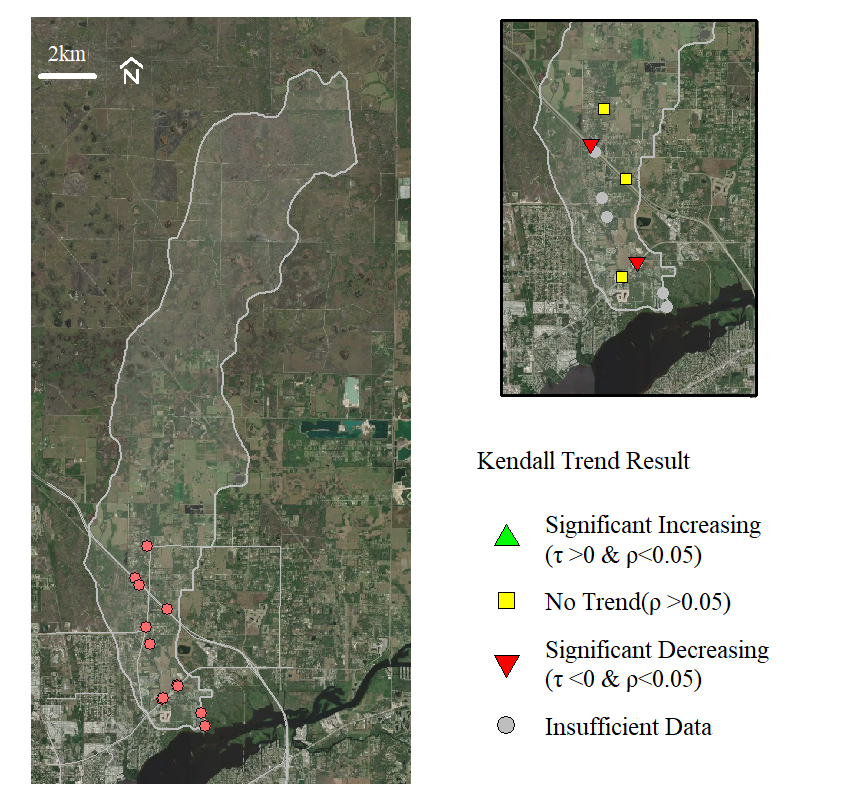
\includegraphics[width=1\linewidth]{C:/Julian_LaCie/_GitHub/SFL_DOSSAC/Plots/WBID3240F_trendmap} \caption{\label{fig:mapfig1} Monitoring locations and individual station trend results within WBID 3240F - Daughtrey Creek.}\label{fig:unnamed-chunk-3}
\end{figure}

\begin{figure}[H]
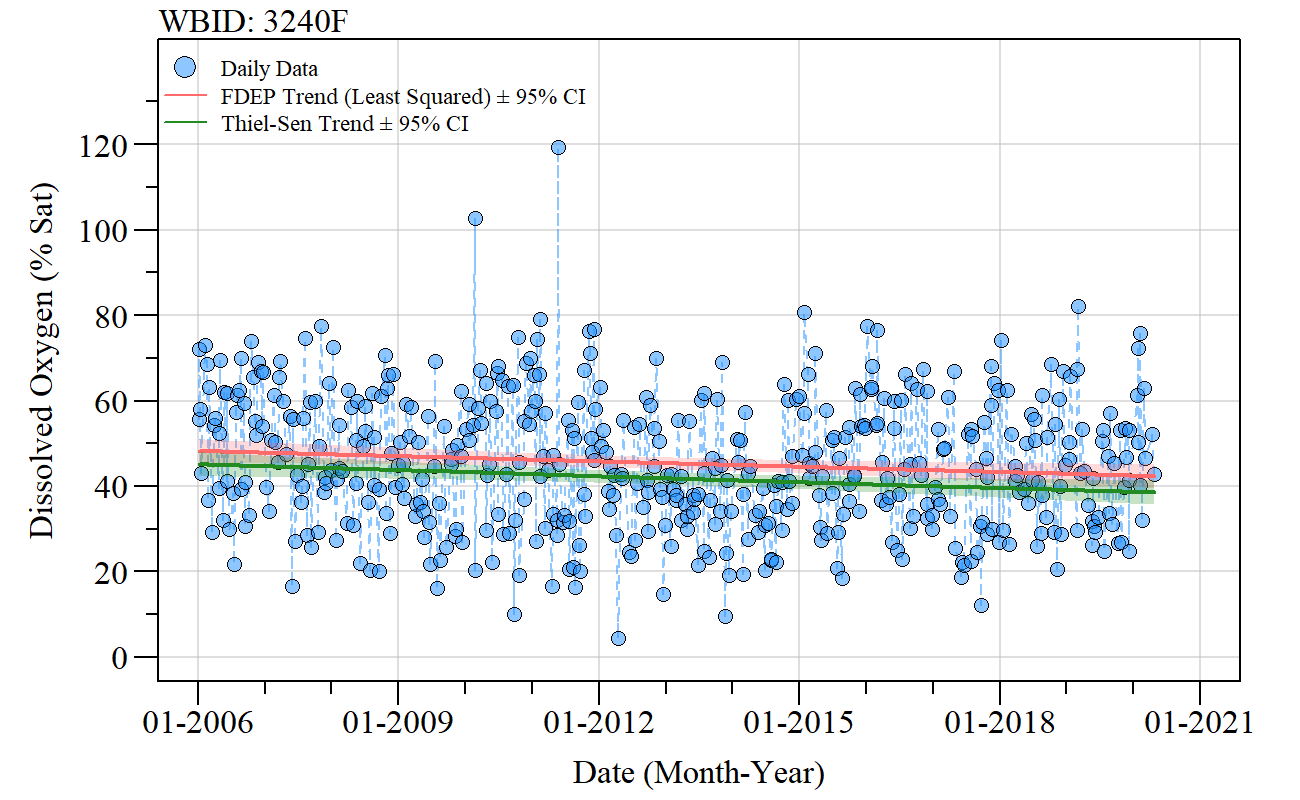
\includegraphics[width=1\linewidth]{C:/Julian_LaCie/_GitHub/SFL_DOSSAC/Plots/WBID3240F_trend} \caption{\label{fig:fig2} Spatially average daily dissolved oxygen percent saturation from Janurary 2006 till December 2020 for  WBID 3240F - Daughtrey Creek. Both least squared (FDEP trend analysis) and Thiel-Sen trends are displayed.}\label{fig:unnamed-chunk-4}
\end{figure}

\begin{figure}[H]

{\centering 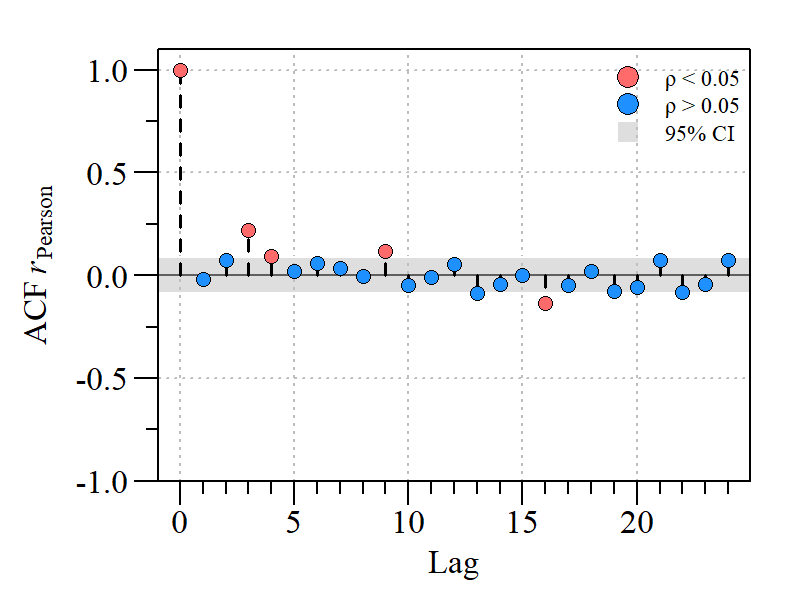
\includegraphics[width=0.75\linewidth]{C:/Julian_LaCie/_GitHub/SFL_DOSSAC/Plots/WBID3240F_trendmodel_ACF} 

}

\caption{\label{fig:fig3} Autocorrelation function (ACF) of least squared trend model residual for the spatially averaged dissolved oxygen time-series. WBID 3240F - Daughtrey Creek.}\label{fig:unnamed-chunk-5}
\end{figure}

\begin{table}[H]

\caption{\label{tab:unnamed-chunk-6}\label{tab:trendtab3} Kendall's trend test results for each individual mointoring locations with suitable data in WBID 3240F - Daughtrey Creek}
\centering
\fontsize{10}{12}\selectfont
\begin{tabular}[t]{lccc}
\toprule
Station ID & Sample Size & Kendall's $\tau$ & $\rho$ -value\\
\midrule
21FLEECO20-29GR & 158 & -0.09 & 0.10\\
21FLEECO20-9GR & 170 & -0.02 & 0.64\\
21FLEECO20A-11GR & 159 & -0.14 & $<$0.01\\
21FLEECO20A-19GR & 148 & -0.03 & 0.56\\
21FLEECOGATRGR91 & 162 & -0.19 & $<$0.01\\
\bottomrule
\end{tabular}
\end{table}

\hypertarget{data-distribution}{%
\subsubsection{Data Distribution}\label{data-distribution}}

The assumption of using a parametric percentile approach, as proposed by
FDEP (2021) is that the data must be normally distributed. Both
Shapiro-Wilk (W=0.99, \(\rho\)\textless0.001) and Anderson-Darling
(A=1.22, \(\rho\)\textless0.01) test indicated that the data was
significantly different from a normal distribution. Moreover,
quantile-quantile and density histogram (Fig \ref{fig:fig4}) indicate a
slight divergence from the normal distribution. Given that the data does
not fit a normal distribution, application of the parametric 10\(^{th}\)
percentile could result in increased Type-II error and an alternative
approach considered.

\begin{figure}[H]

{\centering 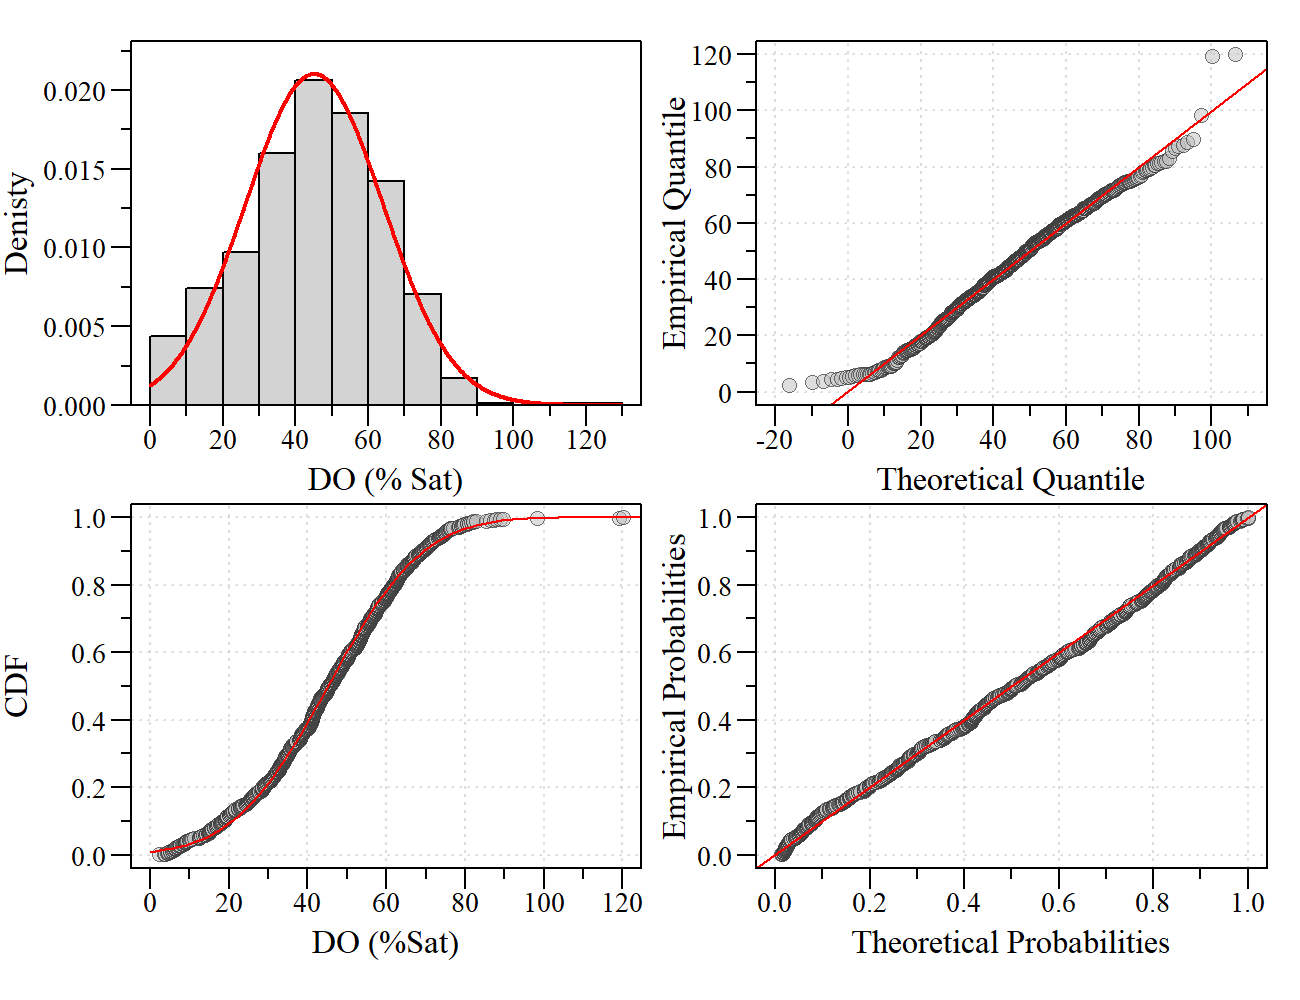
\includegraphics[width=1\linewidth]{C:/Julian_LaCie/_GitHub/SFL_DOSSAC/Plots/WBID3240F_normDist} 

}

\caption{\label{fig:fig4} Evaluation of dissolved oxygen empirical and theoretical normal distribution for Daughtrey Creek (WBID 3240F) during the period of record. Top left: Density histogram of the data compared to the theoretical distribution (red line); Top right: quantile-quantile (Q-Q) plot; Bottom left: cumulative distribution function (CDF) relative to theoretical normal distribution CDF (red line); Bottom right: probability-probability (P-P) plot.}\label{fig:unnamed-chunk-7}
\end{figure}

\hypertarget{popash-creek-wbid-3240q}{%
\subsection{Popash Creek (WBID 3240Q)}\label{popash-creek-wbid-3240q}}

Within the IWR database, WBID 2340Q has a total of 12 sites with DO data
during the period of record (Fig \ref{fig:mapfig5};
\textbf{\protect\hyperlink{appendix-b}{Appendix B}} Table S2). In
evaluating the current data, slight differences in summary statistics
between the FDEP's report (FDEP 2021) and this summary is noted below
for DO in Table \ref{tab:stattab4}. The difference between FDEP's report
and this summary is the inclusion of four additional samples which
slightly change the summary statistics over the period of record. Over
the analysis period of record, two of the 12 monitoring locations
consistently exceed the established DO stream water quality criterion
(Table \ref{tab:tab5}).

\begin{table}[H]

\caption{\label{tab:table2}\label{tab:stattab4} Summary statisic of dissolved oxygen (DO) saturation for Popash Creek (WBID 3240Q) during the period of record (Calendar Year: 2006 - 2020) as reported by FDEP (2021) and summaried data (this report)}
\centering
\resizebox{\linewidth}{!}{
\fontsize{14}{16}\selectfont
\begin{tabular}[t]{>{\raggedright\arraybackslash}p{3cm}lcc>{\centering\arraybackslash}p{1.5cm}>{\centering\arraybackslash}p{3cm}>{\centering\arraybackslash}p{2cm}c>{\centering\arraybackslash}p{2cm}}
\toprule
\textbf{Parameter} & \textbf{Source} & \textbf{Count} & \textbf{Average} & \textbf{Std Dev} & \textbf{10th \%tile} & \textbf{25th \%tile} & \textbf{Median} & \textbf{75th \%tile}\\
\midrule
 & FDEP 2021 & 345 & 45.6 & 18.7 & 20.2¹ / 21.6² & 31.6 & 46.3 & 58.5\\
\cmidrule{2-9}
\multirow{-2}{3cm}{\raggedright\arraybackslash DO Saturation, \%} & This Analysis & 349 & 45.4 & 17.7 & 21.0¹ /22.7² & 31.8 & 46.7 & 58.0\\
\bottomrule
\multicolumn{9}{l}{\rule{0pt}{1em}\textit{Note: }}\\
\multicolumn{9}{l}{\rule{0pt}{1em}Std Dev=Standard Deviation; \%tile=Percentile}\\
\multicolumn{9}{l}{\rule{0pt}{1em}\textsuperscript{1} Percentiles based on ranking of data}\\
\multicolumn{9}{l}{\rule{0pt}{1em}\textsuperscript{2} 10th percentile based on normal distribution using mean and standard deviation}\\
\end{tabular}}
\end{table}

\begin{table}[H]

\caption{\label{tab:unnamed-chunk-8}\label{tab:tab5} Number of years where average dissolved oxygen (DO) saturation values exceed the stream time-of-day DO water quality criteria more than 10\% of the time during the analysis period of record for monitoring locations within wBID 3240Q.}
\centering
\fontsize{8}{10}\selectfont
\begin{tabular}[t]{l>{\centering\arraybackslash}p{2cm}>{\centering\arraybackslash}p{2cm}}
\toprule
\textbf{Station ID} & \textbf{Number of Years WQS Exceeded} & \textbf{Number of Years with Data}\\
\midrule
21FLEECO23-27GR & 15 & 15\\
21FLEECO23-5GR & 10 & 15\\
21FLEECOAC26956 & 0 & 1\\
21FLEECOAD03858 & 0 & 1\\
21FLFTM 28020038 & 0 & 1\\
\addlinespace
21FLFTM 28020232 & 0 & 2\\
21FLFTM CALUSA0020FTM & NA & 1\\
21FLFTM G3SD0079 & 0 & 3\\
21FLGW  45794 & 1 & 1\\
21FLGW  51902 & 0 & 1\\
\addlinespace
21FLGW  53944 & 0 & 1\\
21FLGW  56327 & 0 & 1\\
\bottomrule
\end{tabular}
\end{table}

\hypertarget{trend-analysis-1}{%
\subsubsection{Trend Analysis}\label{trend-analysis-1}}

Similar to Daughtrey creek, the department justified no declining trend
in DO saturation levels using the linear model approach. Using the
linear model approach of trend analysis (Fig \ref{fig:fig6}), the model
had a low degree of fit (R\(^{2}\) = 0.06), significantly
auto-correlated residuals (Statistic = 48.3, df = 3, \(\rho\)
\textless0.001; Fig \ref{fig:fig7}) and the residuals of the model was
significantly different from a normal distribution (W=0.99, \(\rho\)
\textless0.01). The global validation of linear models assumptions
analysis also indicate that the link function, residual kurtosis and
overall assumptions were not satisfied (Global Stat = 13.32, \(\rho\)
\textless0.01). When this same data is evaluated using the Kendall's
correlation test it results in a significant monotonic decline in DO
across the WBID (\(\tau\) = -0.14, \(\rho\) \textless0.001). At
individual monitoring locations, of the two monitoring locations with
sufficient data, both had significantly declining trends while (Table
\ref{tab:trendtab6}). From a seasonal perspective the DO saturation
levels also significantly declined (\(\tau\) = -0.21, \(\rho\)
\textless0.001) at a rate of -0.90 \% DO Yr\(^{-1}\) over the period of
record. From a visual perspective, DO saturation levels were much more
variable and elevated early in the analysis period of record when
comparing later in the period of record(Fig
\textbackslash ref\{fig:fig6{]}). Furthermore, Figure 21 presented by
FDEP 2021, with an extended period of record accentuates this change in
DO condition. The significantly declining trends within and across this
waterbody and the number of sites with a large enough sample size should
be taken into considered when establishing any water quality criterion.
Given these results, setting a DO SSAC for this waterbody could
potentially perpetuating a declining existing condition.

\begin{figure}[H]

{\centering 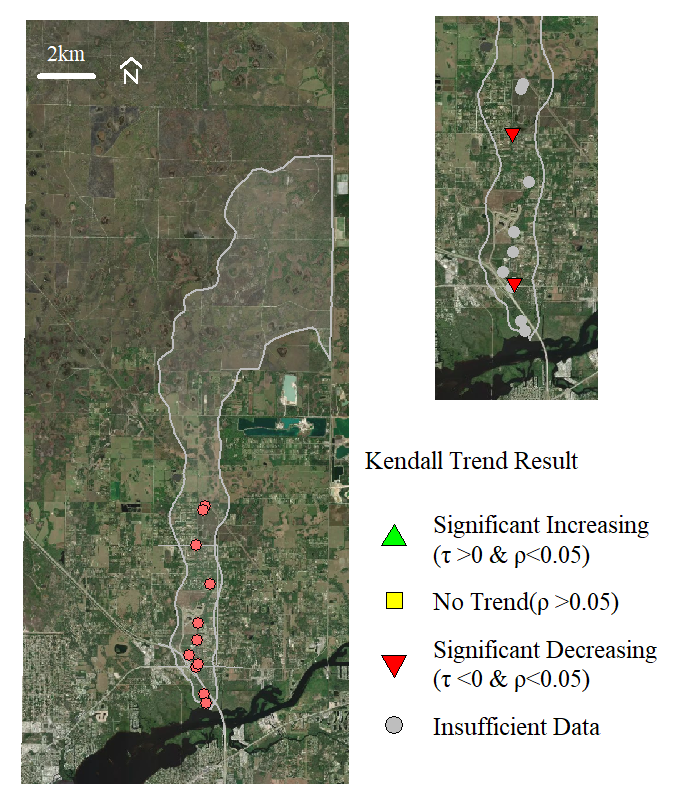
\includegraphics[width=1\linewidth]{C:/Julian_LaCie/_GitHub/SFL_DOSSAC/Plots/WBID3240Q_trendmap} 

}

\caption{\label{fig:mapfig5} Monitoring locations and individual station trend results within WBID 3240Q - Popash Creek.}\label{fig:unnamed-chunk-9}
\end{figure}

\begin{figure}[H]

{\centering 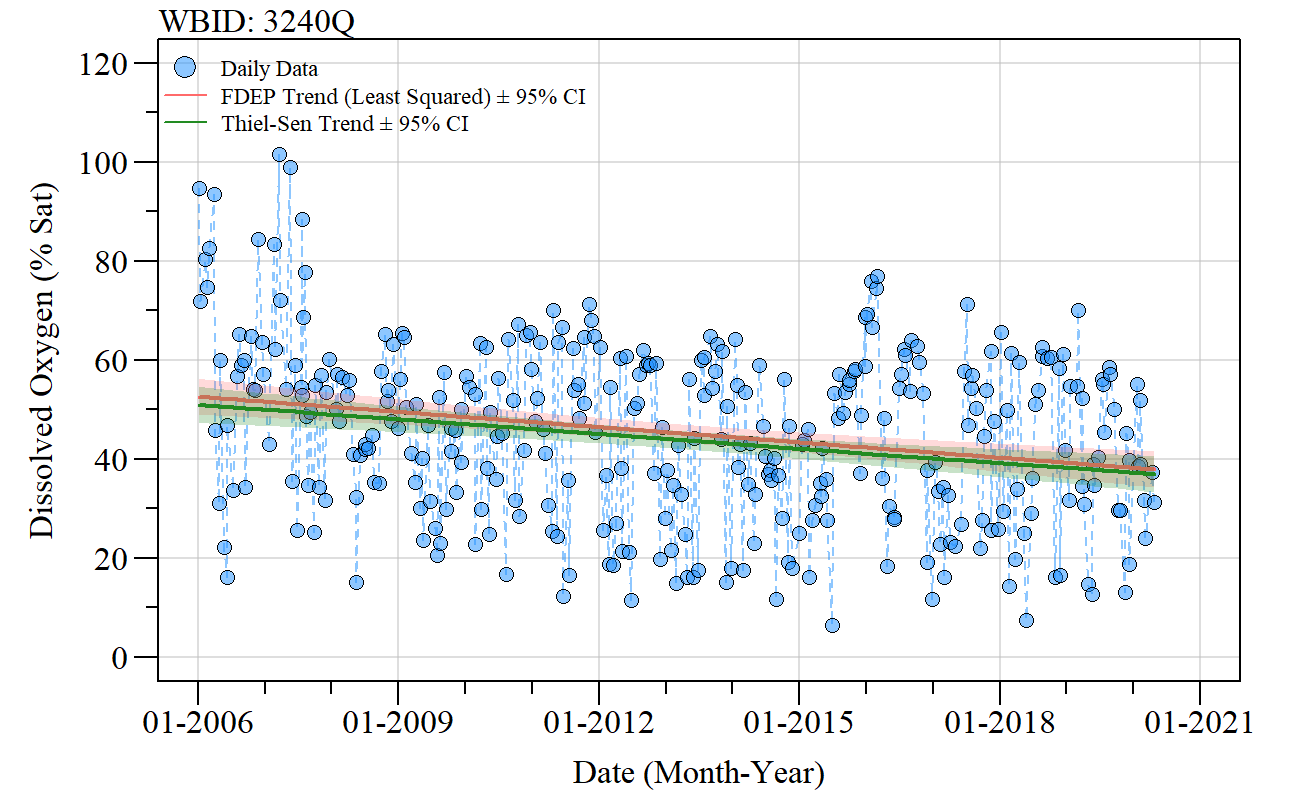
\includegraphics[width=1\linewidth]{C:/Julian_LaCie/_GitHub/SFL_DOSSAC/Plots/WBID3240Q_trend} 

}

\caption{\label{fig:fig6} Spatially average daily dissolved oxygen percent saturation from Janurary 2006 till December 2020 for  WBID 3240Q - Popash Creek. Both least squared (FDEP trend analysis) and Thiel-Sen trends are displayed.}\label{fig:unnamed-chunk-10}
\end{figure}

\begin{figure}[H]

{\centering 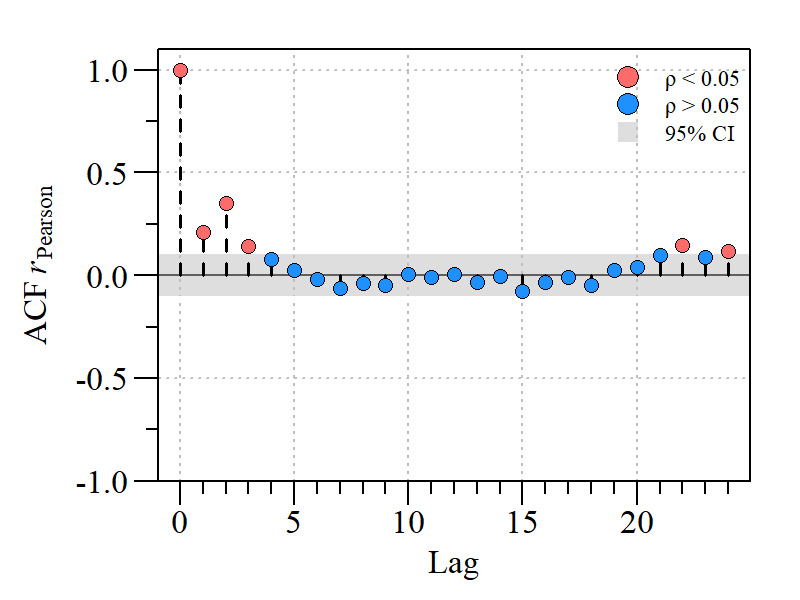
\includegraphics[width=0.75\linewidth]{C:/Julian_LaCie/_GitHub/SFL_DOSSAC/Plots/WBID3240Q_trendmodel_ACF} 

}

\caption{\label{fig:fig7} Autocorrelation function (ACF) of least squared trend model residual for the spatially averaged dissolved oxygen time-series. WBID 3240Q - Popash Creek.}\label{fig:unnamed-chunk-11}
\end{figure}

\begin{table}[H]

\caption{\label{tab:unnamed-chunk-12}\label{tab:trendtab6} Kendall's trend test results for each individual mointoring locations with suitable data in WBID 3240Q - Popash Creek}
\centering
\fontsize{10}{12}\selectfont
\begin{tabular}[t]{lccc}
\toprule
Station ID & Sample Size & Kendall's $\tau$ & $\rho$ -value\\
\midrule
21FLEECO23-27GR & 165 & -0.17 & $<$0.01\\
21FLEECO23-5GR & 170 & -0.14 & $<$0.01\\
\bottomrule
\end{tabular}
\end{table}

\hypertarget{data-distribution-1}{%
\subsubsection{Data Distribution}\label{data-distribution-1}}

Both Shapiro-Wilk (W=0.99, \(\rho\)\textless0.001) and Anderson-Darling
(A=1.74, \(\rho\)\textless0.001) test indicated that the data was
significantly different from a normal distribution. Moreover,
quantile-quantile, cumulative distribution function and density
histogram (Fig \ref{fig:fig8}) indicate a divergence from a normal
distribution. Given that the data does not fit a normal distribution,
application of the parametric 10\(^{th}\) percentile could result in
increased Type-II error and an alternative approach considered.

\begin{figure}[H]

{\centering 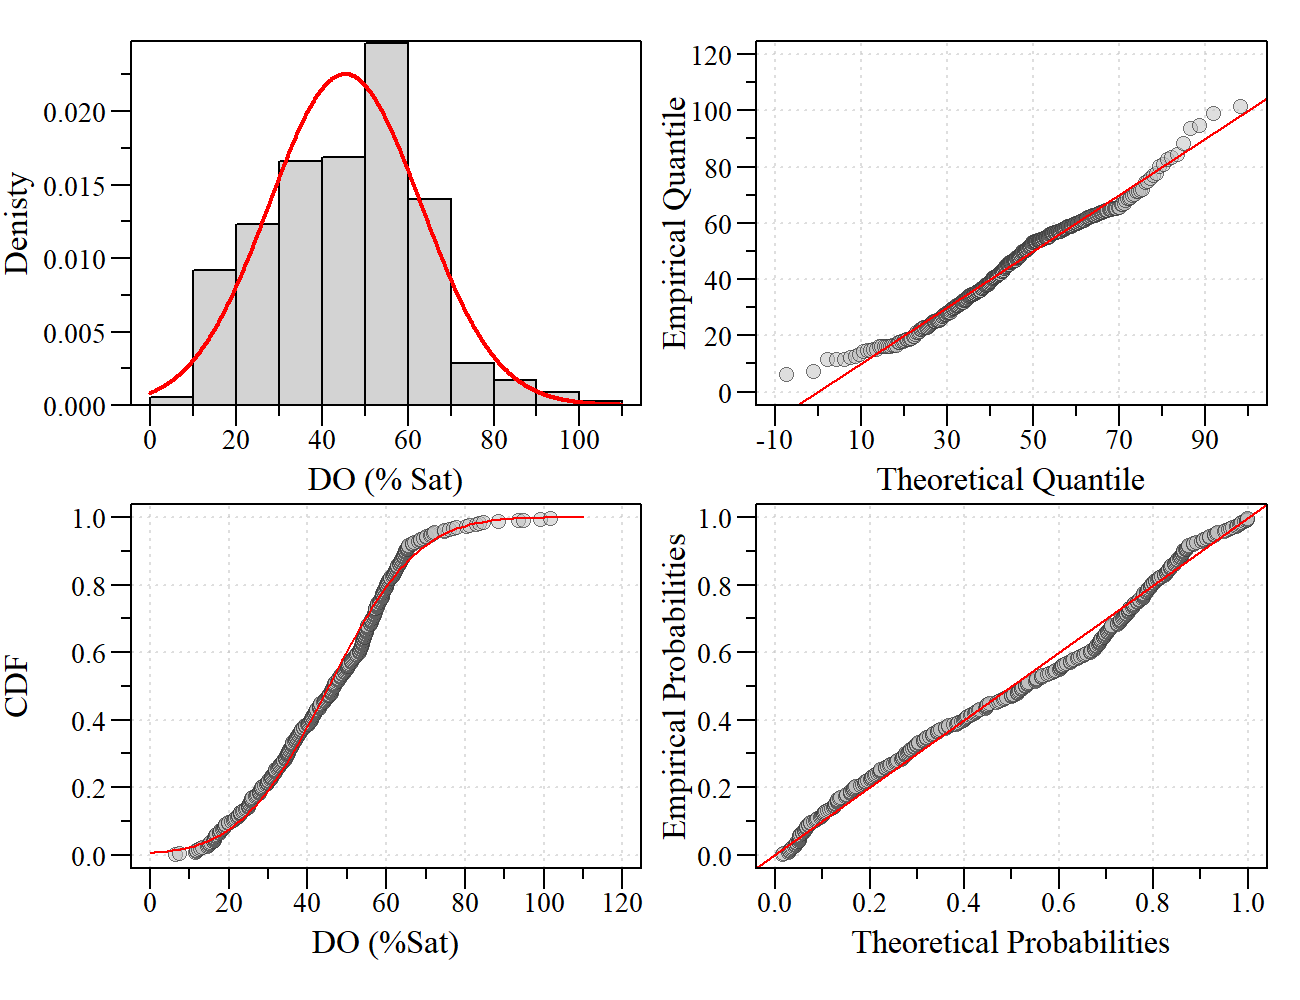
\includegraphics[width=1\linewidth]{C:/Julian_LaCie/_GitHub/SFL_DOSSAC/Plots/WBID3240Q_normDist} 

}

\caption{\label{fig:fig8} Evaluation of dissolved oxygen empirical and theoretical normal distribution for Popash Creek (WBID 3240Q) during the period of record. Top left: Density histogram of the data compared to the theoretical distribution (red line); Top right: quantile-quantile (Q-Q) plot; Bottom left: cumulative distribution function (CDF) relative to theoretical normal distribution CDF (red line); Bottom right: probability-probability (P-P) plot.}\label{fig:unnamed-chunk-13}
\end{figure}

\hypertarget{cypress-creek-wbid-3235c}{%
\subsection{Cypress Creek (WBID 3235C)}\label{cypress-creek-wbid-3235c}}

Within the IWR database, WBID 3235C has a total of 11 sites with DO data
during the period of record, seven of which are located within Cypress
Creek (Fig \ref{fig:mapfig9};
\textbf{\protect\hyperlink{appendix-b}{Appendix B}} Table S3). However,
Figure 23 in the FDEP report only indicates potentially four monitoring
locations. Given these data discrepancies Table \ref{tab:stattab7}
includes all available data within the waterbody compared to values
reported by FDEP (FDEP 2021). Given the disparity between what is
presented in the report and what is available in the IWR database, it is
unclear as to what data was used to derive the proposed DO SSAC for
Cypress Creek (WBID 3235C). Over the analysis period of record given the
limited data, two of the 11 monitoring locations consistently exceed the
established DO stream water quality criterion. The remaining monitoring
locations within Cypress Creek proper and locations across the waterbody
had limited annual data with the exception of 21FLEECOSPANISHGR (Table
\ref{tab:tab8}).

\begin{table}[H]

\caption{\label{tab:unnamed-chunk-14}\label{tab:stattab7} Summary statisic of dissolved oxygen (DO) saturation for Cypress Creek (WBID 3235C) during the period of record (Calendar Year: 2006 - 2020) as reported by FDEP (2021) and summaried data (this report)}
\centering
\resizebox{\linewidth}{!}{
\fontsize{14}{16}\selectfont
\begin{tabular}[t]{>{\raggedright\arraybackslash}p{3cm}lcc>{\centering\arraybackslash}p{1.5cm}>{\centering\arraybackslash}p{3cm}>{\centering\arraybackslash}p{2cm}c>{\centering\arraybackslash}p{2cm}}
\toprule
\textbf{Parameter} & \textbf{Source} & \textbf{Count} & \textbf{Average} & \textbf{Std Dev} & \textbf{10th \%tile} & \textbf{25th \%tile} & \textbf{Median} & \textbf{75th \%tile}\\
\midrule
 & FDEP 2021 & 379 & 48.6 & 15.8 & 28.6¹ / 28.4² & 37.0 & 49.4 & 59.5\\
\cmidrule{2-9}
\multirow{-2}{3cm}{\raggedright\arraybackslash DO Saturation, \%} & This Analysis & 530 & 53.4 & 17.8 & 31.9¹ /30.7² & 40.3 & 53.3 & 65.0\\
\bottomrule
\multicolumn{9}{l}{\rule{0pt}{1em}\textit{Note: }}\\
\multicolumn{9}{l}{\rule{0pt}{1em}Std Dev=Standard Deviation; \%tile=Percentile}\\
\multicolumn{9}{l}{\rule{0pt}{1em}\textsuperscript{1} Percentiles based on ranking of data}\\
\multicolumn{9}{l}{\rule{0pt}{1em}\textsuperscript{2} 10th percentile based on normal distribution using mean and standard deviation}\\
\end{tabular}}
\end{table}

\begin{table}[H]

\caption{\label{tab:unnamed-chunk-15}\label{tab:tab8} Number of years where average dissolved oxygen (DO) saturation values exceed the stream time-of-day DO water quality criteria more than 10\% of the time during the analysis period of record for monitoring locations within wBID 3235C.}
\centering
\fontsize{8}{10}\selectfont
\begin{tabular}[t]{l>{\centering\arraybackslash}p{2cm}>{\centering\arraybackslash}p{2cm}}
\toprule
\textbf{Station ID} & \textbf{Number of Years WQS Exceeded} & \textbf{Number of Years with Data}\\
\midrule
21FLBABRCYPRESS\_HEAD & 3 & 3\\
21FLBABRCYPRESS\_OUTFLOW & 3 & 4\\
21FLEECOCYPRESSGR & 10 & 15\\
21FLEECOFICHTERSGR & 11 & 15\\
21FLEECOSPANISHGR & 1 & 15\\
\addlinespace
21FLFTM 28020043 & 0 & 1\\
21FLFTM 28020237 & 0 & 2\\
21FLFTM CYPRESSGR & 1 & 1\\
21FLFTM G3SD0084 & 0 & 2\\
21FLGW  53948 & 0 & 1\\
\addlinespace
21FLGW  56335 & 0 & 1\\
\bottomrule
\end{tabular}
\end{table}

\begin{figure}[H]

{\centering 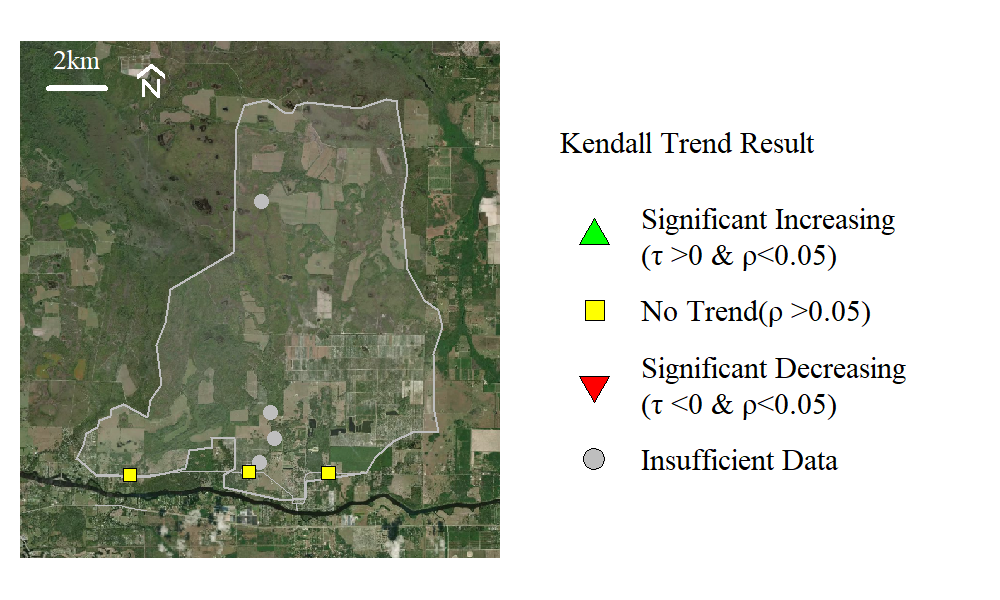
\includegraphics[width=1\linewidth]{C:/Julian_LaCie/_GitHub/SFL_DOSSAC/Plots/WBID3235C_trendmap} 

}

\caption{\label{fig:mapfig9} Monitoring locations and individual station trend results within WBID 3235C - Cypress Creek.}\label{fig:unnamed-chunk-16}
\end{figure}

\hypertarget{trend-analysis-2}{%
\subsubsection{Trend Analysis}\label{trend-analysis-2}}

Using the linear model approach of trend analysis (Fig \ref{fig:fig10}),
the model had a low degree of fit (R\(^{2}\) = 0.02) and significantly
auto-correlated residuals (Statistic = 17.6, df = 3, \(\rho\)
\textless0.001; Fig \ref{fig:fig11}). While the residuals of the trend
model were normally distribution (W=0.99, \(\rho\) = 0.68), the model
did not meet the other assumptions of linear models based on the global
validation of linear models assumptions analysis (Global Stat = 14.80,
\(\rho\) \textless0.01). When evaluated using the Kendall's correlation
test no monotonic trend in DO across the WBID was detected (\(\tau\) =
0.09, \(\rho\) = 0.05) or individual monitoring locations (Table
\ref{tab:trendtab9} and Fig \ref{fig:mapfig9}). From a seasonal
perspective the DO saturation levels had a borderline significantly
increasing trend (\(\tau\) = 0.12, \(\rho\) = 0.05). These results are
for monitoring locations across the waterbody and not Cypress Creek
specifically. However, one monitoring location within Cypress Creek
(21FLEECOCYPRESSGR) did not have a statistically significant monotonic
trend (Table \ref{tab:trendtab9}). Given these results, setting a DO
SSAC for this waterbody could be feasible given the potentially
improving seasonal or a lack of a monotonic trend in DO saturation
levels across the waterbody.

\begin{table}[H]

\caption{\label{tab:unnamed-chunk-17}\label{tab:trendtab9} Kendall's trend test results for each individual mointoring locations with suitable data in WBID 3235C - Cypress Creek}
\centering
\fontsize{10}{12}\selectfont
\begin{tabular}[t]{lccc}
\toprule
Station ID & Sample Size & Kendall's $\tau$ & $\rho$ -value\\
\midrule
21FLEECOCYPRESSGR & 165 & 0.03 & 0.53\\
21FLEECOFICHTERSGR & 166 & 0.01 & 0.85\\
21FLEECOSPANISHGR & 152 & 0.06 & 0.29\\
\bottomrule
\end{tabular}
\end{table}

\begin{figure}[H]

{\centering 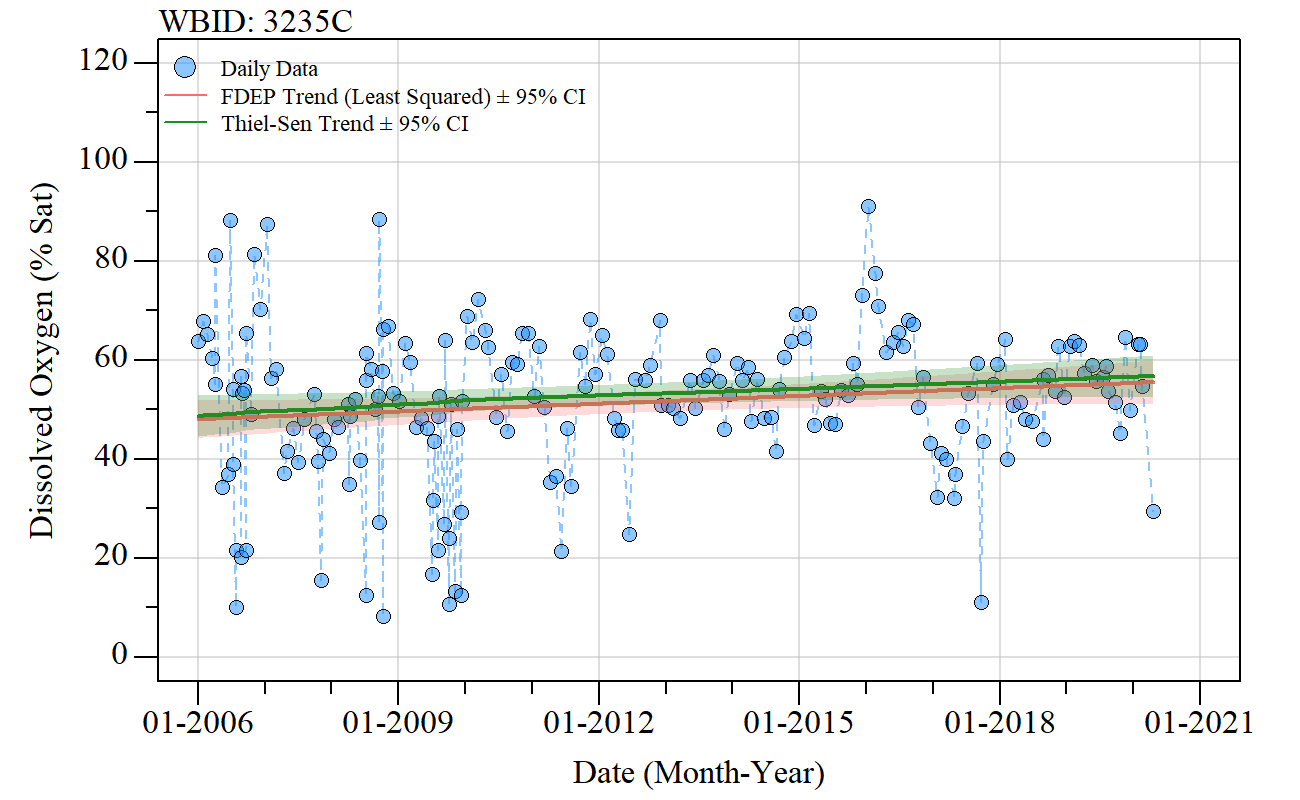
\includegraphics[width=1\linewidth]{C:/Julian_LaCie/_GitHub/SFL_DOSSAC/Plots/WBID3235C_trend} 

}

\caption{\label{fig:fig10} Spatially average daily dissolved oxygen percent saturation from Janurary 2006 till December 2020 for  WBID 3235C - Cypress Creek. Both least squared (FDEP trend analysis) and Thiel-Sen trends are displayed.}\label{fig:unnamed-chunk-18}
\end{figure}

\begin{figure}[H]

{\centering 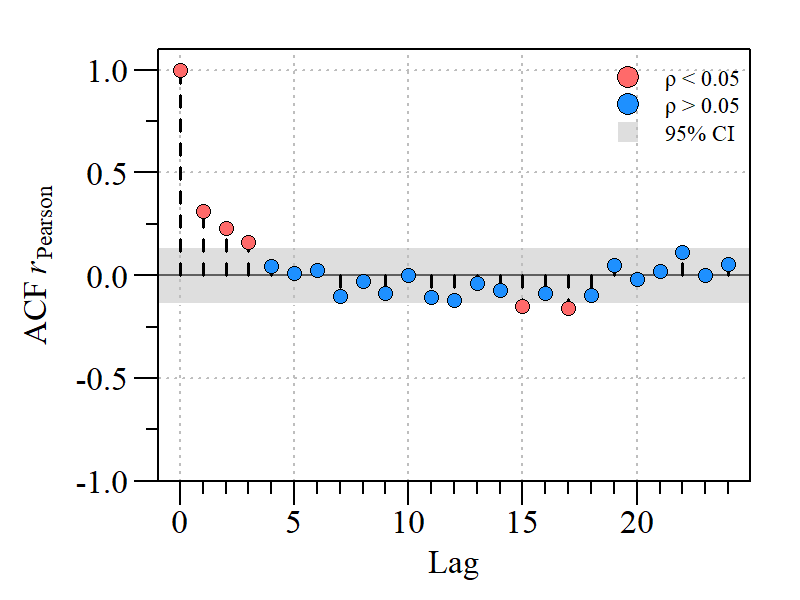
\includegraphics[width=0.75\linewidth]{C:/Julian_LaCie/_GitHub/SFL_DOSSAC/Plots/WBID3235C_trendmodel_ACF} 

}

\caption{\label{fig:fig11} Autocorrelation function (ACF) of least squared trend model residual for the spatially averaged dissolved oxygen time-series. WBID 3235C - Cypress Creek.}\label{fig:unnamed-chunk-19}
\end{figure}

\hypertarget{data-distribution-2}{%
\subsubsection{Data Distribution}\label{data-distribution-2}}

Including all the data across the waterbody, DO saturation levels are
not significantly different from a normal distribution based on the
Shapiro-Wilk (W=1.00, \(\rho\)=0.47) and Anderson-Darling (A=0.37,
\(\rho\)=0.43) normality tests (Fig \ref{fig:fig12}). However, if only
monitoring locations within Cypress Creek (See
\textbf{\protect\hyperlink{appendix-b}{Appendix B}}, Table S3) were
used, DO saturation levels are significantly different from a normal
distribution (Shapiro-Wilk: W=0.99, \(\rho\)\textless0.05;
Anderson-Darling: A=1.00, \(\rho\)\textless0.05; Fig \ref{fig:fig13}).
If monitoring locations within Cypress Creek proper were considered to
develop the DO SSAC, the data do not fit a normal distribution,
application of the parametric 10\(^{th}\) percentile could result in
increased Type-II error and an alternative approach considered.

\begin{figure}[H]

{\centering 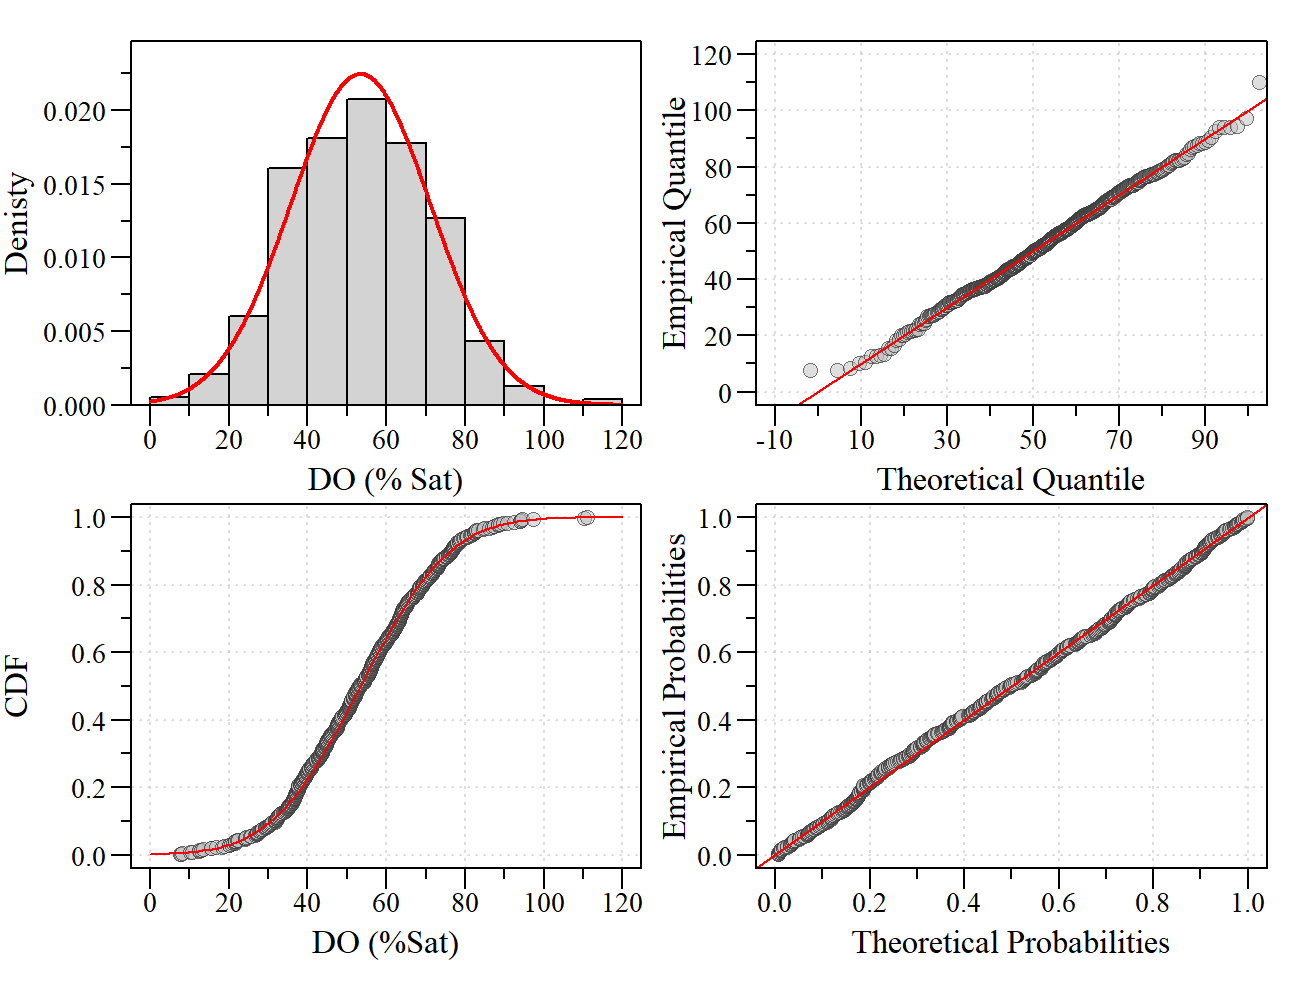
\includegraphics[width=1\linewidth]{C:/Julian_LaCie/_GitHub/SFL_DOSSAC/Plots/WBID3235C_normDist} 

}

\caption{\label{fig:fig12} Evaluation of dissolved oxygen empirical and theoretical normal distribution for all monitoring locations across the Cypress Creek waterbody (WBID 3235C) during the period of record. Top left: Density histogram of the data compared to the theoretical distribution (red line); Top right: quantile-quantile (Q-Q) plot; Bottom left: cumulative distribution function (CDF) relative to theoretical normal distribution CDF (red line); Bottom right: probability-probability (P-P) plot.}\label{fig:unnamed-chunk-20}
\end{figure}

\begin{figure}[H]

{\centering 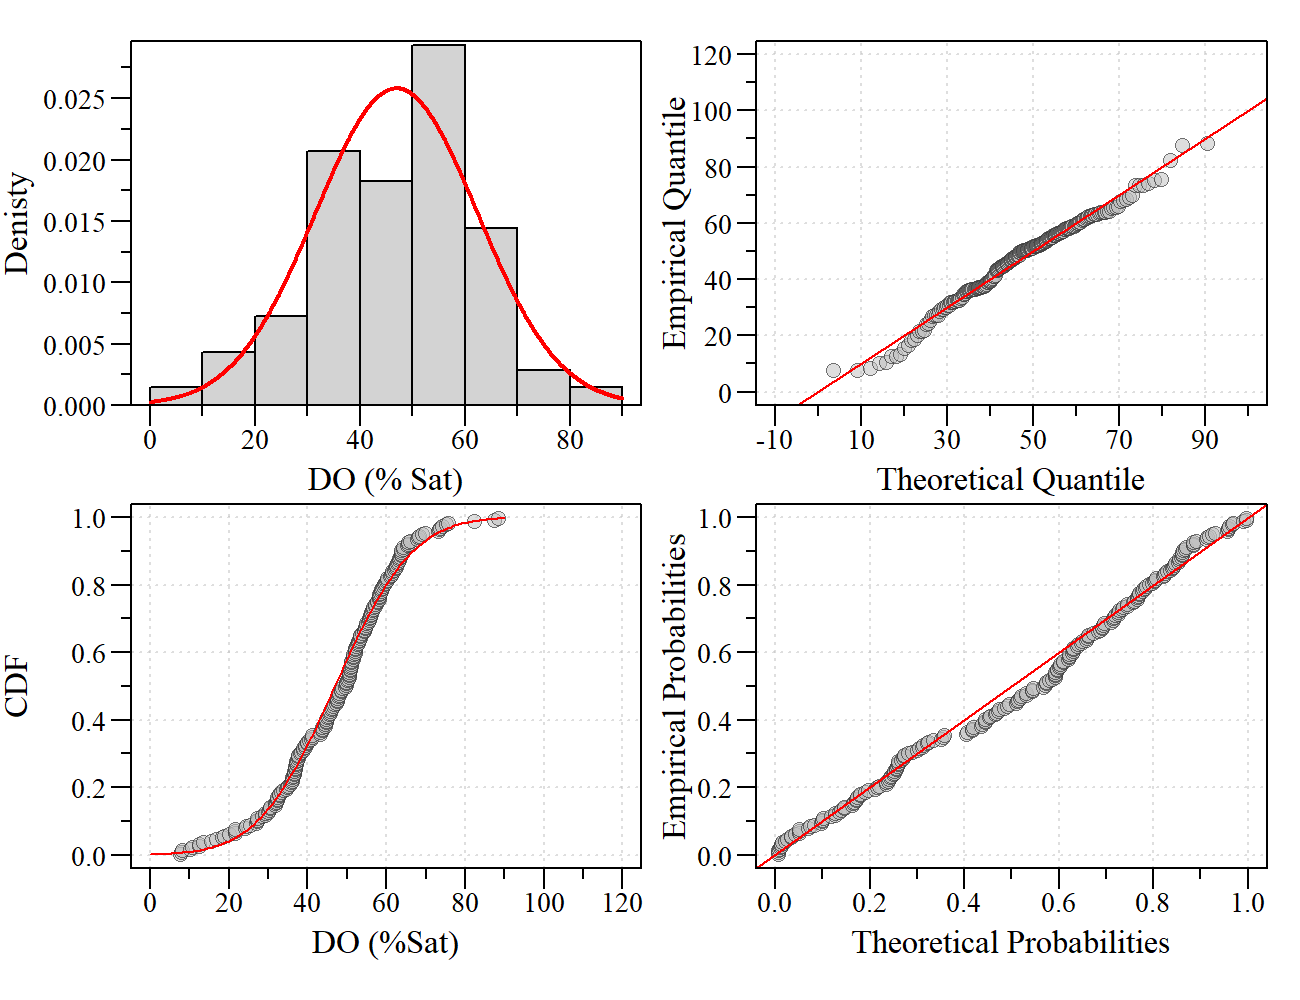
\includegraphics[width=1\linewidth]{C:/Julian_LaCie/_GitHub/SFL_DOSSAC/Plots/WBID3235C_normDist_CCsitesOnly} 

}

\caption{\label{fig:fig13} Evaluation of dissolved oxygen empirical and theoretical normal distribution for for only mointoring locations within Cypress Creek (WBID 3235C; see \textbf{Appendix B}) during the period of record. Top left: Density histogram of the data compared to the theoretical distribution (red line); Top right: quantile-quantile (Q-Q) plot; Bottom left: cumulative distribution function (CDF) relative to theoretical normal distribution CDF (red line); Bottom right: probability-probability (P-P) plot.}\label{fig:unnamed-chunk-21}
\end{figure}

\hypertarget{conclusions}{%
\section{Conclusions}\label{conclusions}}

\begin{itemize}
\item
  This report only evaluated three of the eight waterbodies proposed DO
  SSACs by the Department (FDEP 2021).
\item
  Based on the analysis presented here, Daughtrey and Popash creek have
  significantly declining trends in DO saturation levels averaged across
  the waterbodies and at individual stations.
\item
  In evaluating the data used to propose the DO SSACs, the data do not
  fit the assumptions of the parametric percentile statistic therefore
  alternative methods should be considered to reduce both Type I and II
  errors.
\item
  Given that significantly declining trends were detected, the central
  tendency of the data across the period of record is above the current
  DO criterion and the data does not fit the assumptions of the
  parametric percentile approach, it is recommended that an alternative
  approach be considered for Daughtrey and Popash creek.
\item
  Based on discrepancies between what was reported by FDEP and the
  available data in the IWR database additional analysis and
  documentation is recommended for Cypress Creek (WBID 3235C). Moreover,
  additional clarity is needed in what data was used in the derivation
  of the proposed Cypress Creek DO SSAC. If data outside of Cypress
  Creek was used in the derivation of the criterion this could result in
  increased Type I error.
\item
  While not evaluated in this report, FDEP recommends the adoption of
  the proposed DO SSACs for these waterbodies as \emph{``each waterbody
  supports a healthy biological community as indicated by passing Stream
  Condition Index (SCI) scores, and each waterbody has a high percentage
  of natural lands, such as wetlands and forests, and are not highly
  influenced by anthropogenic inputs.''} However, the SCI data presented
  in Appendix A of the FDEP report (FDEP 2021) is very limited and is
  temporally and spatially limited.
\item
  Not presented in this report, it would appear that several of the
  monitoring locations within each waterbody exceeds either the total
  phosphorus or total nitrogen NNC
  (\href{https://www.flrules.org/gateway/ruleno.asp?id=62-302.531}{62-302.531}(2)(c)2
  FAC) during the evaluation period of record. It is recommended that an
  assessment be conducted to ensure that nutrient conditions are not
  contributing to degraded DO conditions within these waterbodies prior
  proposing alternative DO criterion.
\end{itemize}

\hypertarget{references}{%
\section{References}\label{references}}

\begin{itemize}
\item
  Delignette-Muller M, Dutang C (2015) Fitdistrplus: An R Package for
  Fitting Distributions. Journal of Statistical Software 64:1--34. doi:
  10.18637/jss.v064.i04
\item
  FDEP (2021) DRAFT Evaluation of Waters for Dissolved Oxygen Site
  Specific Alternative Criteria (SSAC) Development. Florida Department
  of Environmental Protection, Tallahassee, FL 85.
\item
  Gross J, Ligges U (2015) nortest: Tests for Normality.
\item
  Helsel DR, Hirsch RM (2002) Statistical methods in water resources.
  United States Geological Survey, Washington DC.
\item
  Millard SP (2013) EnvStats: An R Package for Environmental Statistics,
  2nd edn. doi: 10.1007/978-1-4614-8456-1
\item
  Mohd Razali N, Yap B (2011) Power Comparisons of Shapiro-Wilk,
  Kolmogorov-Smirnov, Lilliefors and Anderson-Darling Tests. Journal of
  Statistical Modeling and Analytics 2:21--33.
\item
  Peña EA, Slate EH (2006) Global Validation of Linear Model
  Assumptions. Journal of the American Statistical Association
  101:341--354. doi: 10.1198/016214505000000637
\item
  Zeileis A, Hothorn T (2002) Diagnostic Checking in Regression
  Relationships. R News 2:7--10.
\end{itemize}

\newpage

\hypertarget{appendix-a}{%
\section{Appendix A}\label{appendix-a}}

\begin{itemize}
\item
  The \texttt{AnalystHelper} \texttt{R}-package documentation can be
  found on Github
  (\url{https://github.com/SwampThingPaul/AnalystHelper}). All other
  packages are available on \href{https://cran.r-project.org/}{CRAN}.
\item
  Data used in this assessment was retrieved from FDEP's IWR database
  found here: \url{http://publicfiles.dep.state.fl.us/DEAR/IWR/}.
\end{itemize}

\begin{center}\rule{0.5\linewidth}{0.5pt}\end{center}

\texttt{R} code used in this analysis.

\begin{Shaded}
\begin{Highlighting}[]
\CommentTok{\# Libraries}
\FunctionTok{library}\NormalTok{(AnalystHelper)}
\FunctionTok{library}\NormalTok{(plyr)}
\FunctionTok{library}\NormalTok{(reshape2)}
\FunctionTok{library}\NormalTok{(openxlsx)}
\FunctionTok{library}\NormalTok{(zoo)}
\FunctionTok{library}\NormalTok{(EnvStats)}
\FunctionTok{library}\NormalTok{(lmtest)}
\FunctionTok{library}\NormalTok{(nortest)}
\FunctionTok{library}\NormalTok{(gvlma)}

\NormalTok{data.path}\OtherTok{=}\StringTok{"./iwr2020\_run60\_2020{-}10{-}05/"}

\CommentTok{\# {-}{-}{-}{-}{-}{-}{-}{-}{-}{-}{-}{-}{-}{-}{-}{-}{-}{-}{-}{-}{-}{-}{-}{-}{-}{-}{-}{-}{-}{-}{-}{-}{-}{-}{-}{-}{-}{-}{-}{-}{-}{-}{-}{-}{-}{-}{-}{-}{-}{-}{-}{-}{-}{-}{-}{-}{-}{-}{-}{-}{-}{-}{-}{-}{-}{-}{-}}
\NormalTok{dat.qual}\OtherTok{=}\FunctionTok{data.frame}\NormalTok{(}\AttributeTok{QUALIFIER=}\FunctionTok{c}\NormalTok{(}\ConstantTok{NA}\NormalTok{,}\StringTok{"!"}\NormalTok{,}\StringTok{"A"}\NormalTok{,}\StringTok{"D"}\NormalTok{,}\StringTok{"E"}\NormalTok{,}\StringTok{"F"}\NormalTok{,}\StringTok{"I"}\NormalTok{,}\StringTok{"R"}\NormalTok{,}\StringTok{"T"}\NormalTok{,}\StringTok{"U"}
\NormalTok{                                ,}\StringTok{"*"}\NormalTok{,}\StringTok{"?"}\NormalTok{,}\StringTok{"B"}\NormalTok{,}\StringTok{"H"}\NormalTok{,}\StringTok{"J"}\NormalTok{,}\StringTok{"K"}\NormalTok{,}\StringTok{"L"}\NormalTok{,}\StringTok{"M"}\NormalTok{,}\StringTok{"N"}\NormalTok{,}
                                \StringTok{"O"}\NormalTok{,}\StringTok{"Q"}\NormalTok{,}\StringTok{"V"}\NormalTok{,}\StringTok{"Y"}\NormalTok{,}\StringTok{"Z"}\NormalTok{),}
                    \AttributeTok{FATALYN=}\FunctionTok{c}\NormalTok{(}\StringTok{"N"}\NormalTok{,}\FunctionTok{rep}\NormalTok{(}\StringTok{"N"}\NormalTok{,}\DecValTok{9}\NormalTok{),}\FunctionTok{rep}\NormalTok{(}\StringTok{"Y"}\NormalTok{,}\DecValTok{14}\NormalTok{)))}

\CommentTok{\# WBID3240F {-} Daughtrey {-}{-}{-}{-}{-}{-}{-}{-}{-}{-}{-}{-}{-}{-}{-}{-}{-}{-}{-}{-}{-}{-}{-}{-}{-}{-}{-}{-}{-}{-}{-}{-}{-}{-}{-}{-}{-}{-}{-}{-}{-}{-}{-}{-}}
\CommentTok{\# Data exported from the IWR database as an xlsx file}
\NormalTok{dat3240F}\OtherTok{=}\FunctionTok{read.xlsx}\NormalTok{(}\FunctionTok{paste0}\NormalTok{(data.path,}\StringTok{"periodOfRecordData3240F.xlsx"}\NormalTok{))}
\NormalTok{dat3240F}\SpecialCharTok{$}\NormalTok{date}\OtherTok{=}\FunctionTok{date.fun}\NormalTok{(}\FunctionTok{convertToDate}\NormalTok{(dat3240F}\SpecialCharTok{$}\NormalTok{date))}
\NormalTok{dat3240F}\OtherTok{=}\FunctionTok{subset}\NormalTok{(dat3240F,year}\SpecialCharTok{\%in\%}\FunctionTok{seq}\NormalTok{(}\DecValTok{2006}\NormalTok{,}\DecValTok{2020}\NormalTok{,}\DecValTok{1}\NormalTok{))}
\CommentTok{\# site not included in original analysis}
\NormalTok{dat3240F}\OtherTok{=}\FunctionTok{subset}\NormalTok{(dat3240F,station.id}\SpecialCharTok{!=}\StringTok{"112WRD 264140081494600"}\NormalTok{);}

\CommentTok{\# QA/QC qualifiers }
\FunctionTok{unique}\NormalTok{(dat3240F}\SpecialCharTok{$}\NormalTok{rcode)}
\FunctionTok{unique}\NormalTok{(dat3240F}\SpecialCharTok{$}\NormalTok{xcode)}
\NormalTok{quals}\OtherTok{=}\FunctionTok{as.character}\NormalTok{(}\FunctionTok{unique}\NormalTok{(dat3240F}\SpecialCharTok{$}\NormalTok{xcode))}
\NormalTok{spl}\OtherTok{=}\FunctionTok{strsplit}\NormalTok{(quals,}\AttributeTok{split=}\StringTok{""}\NormalTok{)}
\NormalTok{quals}\OtherTok{=}\FunctionTok{data.frame}\NormalTok{(}\AttributeTok{xcode=}\NormalTok{quals,}
                 \AttributeTok{q1=}\FunctionTok{sapply}\NormalTok{(spl,}\StringTok{"["}\NormalTok{,}\DecValTok{1}\NormalTok{),}
                 \AttributeTok{q2=}\FunctionTok{sapply}\NormalTok{(spl,}\StringTok{"["}\NormalTok{,}\DecValTok{2}\NormalTok{),}
                 \AttributeTok{q3=}\FunctionTok{sapply}\NormalTok{(spl,}\StringTok{"["}\NormalTok{,}\DecValTok{3}\NormalTok{))}
\NormalTok{quals}\SpecialCharTok{$}\NormalTok{Fatal}\OtherTok{=}\FunctionTok{with}\NormalTok{(quals,}
                 \FunctionTok{ifelse}\NormalTok{(q1}\SpecialCharTok{\%in\%}\FunctionTok{subset}\NormalTok{(dat.qual,FATALYN}\SpecialCharTok{==}\StringTok{"Y"}\NormalTok{)}\SpecialCharTok{$}\NormalTok{QUALIFIER}\SpecialCharTok{|}
\NormalTok{                        q2}\SpecialCharTok{\%in\%}\FunctionTok{subset}\NormalTok{(dat.qual,FATALYN}\SpecialCharTok{==}\StringTok{"Y"}\NormalTok{)}\SpecialCharTok{$}\NormalTok{QUALIFIER}\SpecialCharTok{|}
\NormalTok{                        q3}\SpecialCharTok{\%in\%}\FunctionTok{subset}\NormalTok{(dat.qual,FATALYN}\SpecialCharTok{==}\StringTok{"Y"}\NormalTok{)}\SpecialCharTok{$}\NormalTok{QUALIFIER,}
                        \StringTok{"Y"}\NormalTok{,}\StringTok{"N"}\NormalTok{))}
\NormalTok{dat3240F}\OtherTok{=}\FunctionTok{merge}\NormalTok{(dat3240F,quals[,}\FunctionTok{c}\NormalTok{(}\StringTok{"xcode"}\NormalTok{,}\StringTok{"Fatal"}\NormalTok{)],}\StringTok{"xcode"}\NormalTok{,}\AttributeTok{all.x=}\NormalTok{T)}
\NormalTok{dat3240F}\OtherTok{=}\FunctionTok{subset}\NormalTok{(dat3240F,Fatal}\SpecialCharTok{==}\StringTok{"N"}\NormalTok{)}
\NormalTok{dat3240F}\SpecialCharTok{$}\NormalTok{HalfMDL}\OtherTok{=}\FunctionTok{with}\NormalTok{(dat3240F,}
                      \FunctionTok{ifelse}\NormalTok{(}\FunctionTok{is.na}\NormalTok{(mdl)}\SpecialCharTok{==}\NormalTok{T,result,}
                             \FunctionTok{ifelse}\NormalTok{(result}\SpecialCharTok{\textless{}=}\NormalTok{mdl,result}\SpecialCharTok{/}\DecValTok{2}\NormalTok{,result)))}

\NormalTok{params.keep}\OtherTok{=}\FunctionTok{c}\NormalTok{(}\StringTok{"CHLAC"}\NormalTok{,}\StringTok{"COLOR"}\NormalTok{,}\StringTok{"COND"}\NormalTok{,}
              \StringTok{"DO"}\NormalTok{,}\StringTok{"DOSAT"}\NormalTok{,}\StringTok{"TN"}\NormalTok{,}\StringTok{"TP"}\NormalTok{,}\StringTok{"TOC"}\NormalTok{,}\StringTok{"TEMP"}\NormalTok{)}
\NormalTok{dat3240F.xtab}\OtherTok{=}\FunctionTok{dcast}\NormalTok{(}\FunctionTok{subset}\NormalTok{(dat3240F,master.code}\SpecialCharTok{\%in\%}\NormalTok{params.keep),}
\NormalTok{                              wbid}\SpecialCharTok{+}\NormalTok{station.id}\SpecialCharTok{+}\NormalTok{lat}\SpecialCharTok{+}\NormalTok{long}\SpecialCharTok{+}\NormalTok{date}\SpecialCharTok{\textasciitilde{}}\NormalTok{master.code,}
                              \AttributeTok{value.var=}\StringTok{"HalfMDL"}\NormalTok{,mean)}
\NormalTok{dat3240F.xtab}\SpecialCharTok{$}\NormalTok{Sal}\OtherTok{=}\FunctionTok{with}\NormalTok{(dat3240F.xtab,}\FunctionTok{SalinityCalc}\NormalTok{(COND,TEMP))}
\NormalTok{dat3240F.xtab}\SpecialCharTok{$}\NormalTok{DOsat.calc}\OtherTok{=}\FunctionTok{with}\NormalTok{(dat3240F.xtab,}\FunctionTok{DO\_PerSat}\NormalTok{(TEMP,DO,Sal))}
\NormalTok{dat3240F.xtab}\SpecialCharTok{$}\NormalTok{DoY}\OtherTok{=}\FunctionTok{as.numeric}\NormalTok{(}\FunctionTok{format}\NormalTok{(dat3240F.xtab}\SpecialCharTok{$}\NormalTok{date,}\StringTok{"\%j"}\NormalTok{))}
\NormalTok{dat3240F.xtab}\SpecialCharTok{$}\NormalTok{CY}\OtherTok{=}\FunctionTok{as.numeric}\NormalTok{(}\FunctionTok{format}\NormalTok{(dat3240F.xtab}\SpecialCharTok{$}\NormalTok{date,}\StringTok{"\%Y"}\NormalTok{))}
\NormalTok{dat3240F.xtab}\SpecialCharTok{$}\NormalTok{month}\OtherTok{=}\FunctionTok{as.numeric}\NormalTok{(}\FunctionTok{format}\NormalTok{(dat3240F.xtab}\SpecialCharTok{$}\NormalTok{date,}\StringTok{\textquotesingle{}\%m\textquotesingle{}}\NormalTok{))}

\DocumentationTok{\#\# Spatially Average Data}
\NormalTok{dat3240F.xtab.mean}\OtherTok{=}\FunctionTok{ddply}\NormalTok{(dat3240F.xtab,}\StringTok{"date"}\NormalTok{,summarise,}
                         \AttributeTok{mean.DOSat=}\FunctionTok{mean}\NormalTok{(DOsat.calc,}\AttributeTok{na.rm=}\NormalTok{T))}
\NormalTok{dat3240F.xtab.mean}\SpecialCharTok{$}\NormalTok{DoY}\OtherTok{=}\FunctionTok{as.numeric}\NormalTok{(}\FunctionTok{format}\NormalTok{(dat3240F.xtab.mean}\SpecialCharTok{$}\NormalTok{date,}\StringTok{"\%j"}\NormalTok{))}
\NormalTok{dat3240F.xtab.mean}\SpecialCharTok{$}\NormalTok{CY}\OtherTok{=}\FunctionTok{as.numeric}\NormalTok{(}\FunctionTok{format}\NormalTok{(dat3240F.xtab.mean}\SpecialCharTok{$}\NormalTok{date,}\StringTok{\textquotesingle{}\%Y\textquotesingle{}}\NormalTok{))}
\NormalTok{dat3240F.xtab.mean}\OtherTok{=}\FunctionTok{subset}\NormalTok{(dat3240F.xtab.mean,}\FunctionTok{is.na}\NormalTok{(mean.DOSat)}\SpecialCharTok{==}\NormalTok{F)}
\NormalTok{dat3240F.xtab.mean}\SpecialCharTok{$}\NormalTok{dum.val}\OtherTok{=}\DecValTok{1}\SpecialCharTok{:}\FunctionTok{nrow}\NormalTok{(dat3240F.xtab.mean) }\CommentTok{\#time index}

\CommentTok{\# WQS Eval}
\NormalTok{dat3240F}\SpecialCharTok{$}\NormalTok{time}\OtherTok{=}\FunctionTok{with}\NormalTok{(dat3240F,}\FunctionTok{ifelse}\NormalTok{(}\FunctionTok{nchar}\NormalTok{(time)}\SpecialCharTok{==}\DecValTok{3}\NormalTok{,}
                                   \FunctionTok{paste0}\NormalTok{(}\DecValTok{0}\NormalTok{,time),time))}
\NormalTok{dat3240F}\SpecialCharTok{$}\NormalTok{datetime}\OtherTok{=}\FunctionTok{with}\NormalTok{(dat3240F,}
                       \FunctionTok{date.fun}\NormalTok{(}\FunctionTok{paste}\NormalTok{(date,time),}\AttributeTok{form=}\StringTok{"\%F \%H\%M"}\NormalTok{))}
\NormalTok{dat3240F.xtab2}\OtherTok{=}\FunctionTok{dcast}\NormalTok{(}\FunctionTok{subset}\NormalTok{(dat3240F,}
\NormalTok{                            master.code}\SpecialCharTok{\%in\%}\NormalTok{params.keep}\SpecialCharTok{\&}
\NormalTok{                              station.id}\SpecialCharTok{!=}\StringTok{"112WRD  264140081494600"}\NormalTok{),}
\NormalTok{                     wbid}\SpecialCharTok{+}\NormalTok{station.id}\SpecialCharTok{+}\NormalTok{lat}\SpecialCharTok{+}\NormalTok{long}\SpecialCharTok{+}\NormalTok{datetime}\SpecialCharTok{\textasciitilde{}}\NormalTok{master.code,}
                     \AttributeTok{value.var=}\StringTok{"HalfMDL"}\NormalTok{,mean)}
\NormalTok{dat3240F.xtab2}\SpecialCharTok{$}\NormalTok{CY}\OtherTok{=}\FunctionTok{as.numeric}\NormalTok{(}\FunctionTok{format}\NormalTok{(dat3240F.xtab2}\SpecialCharTok{$}\NormalTok{date,}\StringTok{"\%Y"}\NormalTok{))}
\NormalTok{dat3240F.xtab2}\SpecialCharTok{$}\NormalTok{Sal}\OtherTok{=}\FunctionTok{with}\NormalTok{(dat3240F.xtab2,}\FunctionTok{SalinityCalc}\NormalTok{(COND,TEMP))}
\NormalTok{dat3240F.xtab2}\SpecialCharTok{$}\NormalTok{DOsat.calc}\OtherTok{=}\FunctionTok{with}\NormalTok{(dat3240F.xtab2,}\FunctionTok{DO\_PerSat}\NormalTok{(TEMP,DO,Sal))}
\NormalTok{dat3240F.xtab2}\SpecialCharTok{$}\NormalTok{DO.TOD.WQS}\OtherTok{=}\FunctionTok{with}\NormalTok{(dat3240F.xtab2,}
                               \FunctionTok{DO.TOD.WQS.stream}\NormalTok{(datetime))}
\NormalTok{dat3240F.xtab2}\SpecialCharTok{$}\NormalTok{exceed}\OtherTok{=}\FunctionTok{with}\NormalTok{(dat3240F.xtab2,}
                           \FunctionTok{ifelse}\NormalTok{(DOsat.calc}\SpecialCharTok{\textless{}}\NormalTok{DO.TOD.WQS,}\DecValTok{1}\NormalTok{,}\DecValTok{0}\NormalTok{))}

\NormalTok{rslt}\FloatTok{.3240}\NormalTok{F}\OtherTok{=}\FunctionTok{ddply}\NormalTok{(dat3240F.xtab2,}\FunctionTok{c}\NormalTok{(}\StringTok{"station.id"}\NormalTok{,}\StringTok{"CY"}\NormalTok{),}
\NormalTok{                 summarise,}\AttributeTok{N.exceed=}\FunctionTok{sum}\NormalTok{(exceed,}\AttributeTok{na.rm=}\NormalTok{T),}
                 \AttributeTok{N.val=}\FunctionTok{N.obs}\NormalTok{(DOsat.calc))}
\NormalTok{rslt}\FloatTok{.3240}\NormalTok{F}\SpecialCharTok{$}\NormalTok{PerExceed}\OtherTok{=}\FunctionTok{with}\NormalTok{(rslt}\FloatTok{.3240}\NormalTok{F,N.exceed}\SpecialCharTok{/}\NormalTok{N.val)}\SpecialCharTok{*}\DecValTok{100}
\NormalTok{rslt}\FloatTok{.3240}\NormalTok{F}\SpecialCharTok{$}\NormalTok{status}\OtherTok{=}\FunctionTok{with}\NormalTok{(rslt}\FloatTok{.3240}\NormalTok{F,}\FunctionTok{ifelse}\NormalTok{(PerExceed}\SpecialCharTok{\textgreater{}}\DecValTok{10}\NormalTok{,}\DecValTok{1}\NormalTok{,}\DecValTok{0}\NormalTok{))}
\NormalTok{rslt}\FloatTok{.3240}\NormalTok{F}\OtherTok{=}\FunctionTok{ddply}\NormalTok{(rslt}\FloatTok{.3240}\NormalTok{F,}\StringTok{"station.id"}\NormalTok{,summarise,}
                 \AttributeTok{sum.status=}\FunctionTok{sum}\NormalTok{(status),}\AttributeTok{n.val=}\FunctionTok{N.obs}\NormalTok{(status))}

\CommentTok{\# Kendall Trend}
\NormalTok{ken.rslt}\OtherTok{=}\FunctionTok{with}\NormalTok{(dat3240F.xtab.mean,}
              \FunctionTok{cor.test}\NormalTok{(mean.DOSat,}\FunctionTok{as.numeric}\NormalTok{(date),}\AttributeTok{method=}\StringTok{"kendall"}\NormalTok{))}

\CommentTok{\# Seasonal Kendall}
\NormalTok{dat3240F.xtab.mean.sea}\OtherTok{=}\FunctionTok{ddply}\NormalTok{(dat3240F.xtab,}\FunctionTok{c}\NormalTok{(}\StringTok{"month"}\NormalTok{,}\StringTok{"CY"}\NormalTok{),summarise,}
                             \AttributeTok{mean.DOSat=}\FunctionTok{mean}\NormalTok{(DOsat.calc,}\AttributeTok{na.rm=}\NormalTok{T))}
\NormalTok{sea.rslt}\OtherTok{=}\FunctionTok{kendallSeasonalTrendTest}\NormalTok{(mean.DOSat}\SpecialCharTok{\textasciitilde{}}\NormalTok{month}\SpecialCharTok{+}\NormalTok{CY,}
                                  \AttributeTok{data=}\NormalTok{dat3240F.xtab.mean.sea)}
\FunctionTok{print}\NormalTok{(sea.rslt)}

\CommentTok{\# Individual station Kendall Trend}
\NormalTok{samp.screen}\OtherTok{=}\FunctionTok{ddply}\NormalTok{(dat3240F.xtab,}\StringTok{"station.id"}\NormalTok{,summarise,}
                  \AttributeTok{N.val=}\FunctionTok{N.obs}\NormalTok{(DOsat.calc))}
\NormalTok{samp.screen}\OtherTok{=}\FunctionTok{subset}\NormalTok{(samp.screen,N.val}\SpecialCharTok{\textgreater{}}\DecValTok{20}\NormalTok{)}
\NormalTok{dat3240F.trend}\OtherTok{=}\FunctionTok{subset}\NormalTok{(dat3240F.xtab,}
\NormalTok{                      station.id}\SpecialCharTok{\%in\%}\NormalTok{samp.screen}\SpecialCharTok{$}\NormalTok{station.id)}
\NormalTok{dat3240F.trend}\SpecialCharTok{$}\NormalTok{date.num}\OtherTok{=}\FunctionTok{as.numeric}\NormalTok{(dat3240F.trend}\SpecialCharTok{$}\NormalTok{date)}
\NormalTok{site.trend}\OtherTok{=}\FunctionTok{ddply}\NormalTok{(dat3240F.trend,}\StringTok{"station.id"}\NormalTok{,summarise,}
                 \AttributeTok{N.val=}\FunctionTok{N.obs}\NormalTok{(DOsat.calc,}\StringTok{"NaN"}\NormalTok{),}
                 \AttributeTok{est=}\FunctionTok{cor.test}\NormalTok{(DOsat.calc,date.num,}
                              \AttributeTok{method=}\StringTok{"kendall"}\NormalTok{)}\SpecialCharTok{$}\NormalTok{estimate,}
                 \AttributeTok{pval=}\FunctionTok{cor.test}\NormalTok{(DOsat.calc,date.num,}
                               \AttributeTok{method=}\StringTok{"kendall"}\NormalTok{)}\SpecialCharTok{$}\NormalTok{p.value)}

\CommentTok{\# lm trend}
\NormalTok{dep.trend}\OtherTok{=}\FunctionTok{lm}\NormalTok{(mean.DOSat}\SpecialCharTok{\textasciitilde{}}\NormalTok{date,dat3240F.xtab.mean)}
\FunctionTok{summary}\NormalTok{(dep.trend)}
\FunctionTok{gvlma}\NormalTok{(dep.trend)}
\FunctionTok{layout}\NormalTok{(}\FunctionTok{matrix}\NormalTok{(}\DecValTok{1}\SpecialCharTok{:}\DecValTok{4}\NormalTok{,}\DecValTok{2}\NormalTok{,}\DecValTok{2}\NormalTok{));}\FunctionTok{plot}\NormalTok{(dep.trend)}

\FunctionTok{bgtest}\NormalTok{(dep.trend,}\AttributeTok{order=}\DecValTok{3}\NormalTok{)}
\FunctionTok{shapiro.test}\NormalTok{(}\FunctionTok{residuals}\NormalTok{(dep.trend))}

\DocumentationTok{\#\# Data distribution}
\NormalTok{tmp}\OtherTok{=}\FunctionTok{subset}\NormalTok{(dat3240F.xtab,}\FunctionTok{is.na}\NormalTok{(DOsat.calc)}\SpecialCharTok{==}\NormalTok{F)}\SpecialCharTok{$}\NormalTok{DOsat.calc}
\FunctionTok{shapiro.test}\NormalTok{(tmp)}
\FunctionTok{ad.test}\NormalTok{(tmp)}

\FunctionTok{plotdist}\NormalTok{(tmp,}\StringTok{"norm"}\NormalTok{,}\AttributeTok{para=}\FunctionTok{list}\NormalTok{(}\AttributeTok{mean=}\FunctionTok{mean}\NormalTok{(tmp),}\AttributeTok{sd=}\FunctionTok{sd}\NormalTok{(tmp)))}

\CommentTok{\# WBID3240Q {-} Popash  {-}{-}{-}{-}{-}{-}{-}{-}{-}{-}{-}{-}{-}{-}{-}{-}{-}{-}{-}{-}{-}{-}{-}{-}{-}{-}{-}{-}{-}{-}{-}{-}{-}{-}{-}{-}{-}{-}{-}{-}{-}{-}{-}{-}{-}{-}}
\NormalTok{dat3240Q}\OtherTok{=}\FunctionTok{read.xlsx}\NormalTok{(}\FunctionTok{paste0}\NormalTok{(data.path,}\StringTok{"periodOfRecordData3240Q.xlsx"}\NormalTok{))}
\NormalTok{dat3240Q}\SpecialCharTok{$}\NormalTok{date}\OtherTok{=}\FunctionTok{date.fun}\NormalTok{(}\FunctionTok{convertToDate}\NormalTok{(dat3240Q}\SpecialCharTok{$}\NormalTok{date))}
\NormalTok{dat3240Q}\OtherTok{=}\FunctionTok{subset}\NormalTok{(dat3240Q,year}\SpecialCharTok{\%in\%}\FunctionTok{seq}\NormalTok{(}\DecValTok{2006}\NormalTok{,}\DecValTok{2020}\NormalTok{,}\DecValTok{1}\NormalTok{))}

\CommentTok{\# QA/QC qualifiers }
\FunctionTok{unique}\NormalTok{(dat3240Q}\SpecialCharTok{$}\NormalTok{rcode)}
\FunctionTok{unique}\NormalTok{(dat3240Q}\SpecialCharTok{$}\NormalTok{xcode)}
\NormalTok{quals}\OtherTok{=}\FunctionTok{as.character}\NormalTok{(}\FunctionTok{unique}\NormalTok{(dat3240Q}\SpecialCharTok{$}\NormalTok{xcode))}
\NormalTok{spl}\OtherTok{=}\FunctionTok{strsplit}\NormalTok{(quals,}\AttributeTok{split=}\StringTok{""}\NormalTok{)}
\NormalTok{quals}\OtherTok{=}\FunctionTok{data.frame}\NormalTok{(}\AttributeTok{xcode=}\NormalTok{quals,}
                 \AttributeTok{q1=}\FunctionTok{sapply}\NormalTok{(spl,}\StringTok{"["}\NormalTok{,}\DecValTok{1}\NormalTok{),}
                 \AttributeTok{q2=}\FunctionTok{sapply}\NormalTok{(spl,}\StringTok{"["}\NormalTok{,}\DecValTok{2}\NormalTok{),}
                 \AttributeTok{q3=}\FunctionTok{sapply}\NormalTok{(spl,}\StringTok{"["}\NormalTok{,}\DecValTok{3}\NormalTok{))}
\NormalTok{quals}\SpecialCharTok{$}\NormalTok{Fatal}\OtherTok{=}\FunctionTok{with}\NormalTok{(quals,}
                 \FunctionTok{ifelse}\NormalTok{(q1}\SpecialCharTok{\%in\%}\FunctionTok{subset}\NormalTok{(dat.qual,FATALYN}\SpecialCharTok{==}\StringTok{"Y"}\NormalTok{)}\SpecialCharTok{$}\NormalTok{QUALIFIER}\SpecialCharTok{|}
\NormalTok{                        q2}\SpecialCharTok{\%in\%}\FunctionTok{subset}\NormalTok{(dat.qual,FATALYN}\SpecialCharTok{==}\StringTok{"Y"}\NormalTok{)}\SpecialCharTok{$}\NormalTok{QUALIFIER}\SpecialCharTok{|}
\NormalTok{                        q3}\SpecialCharTok{\%in\%}\FunctionTok{subset}\NormalTok{(dat.qual,FATALYN}\SpecialCharTok{==}\StringTok{"Y"}\NormalTok{)}\SpecialCharTok{$}\NormalTok{QUALIFIER,}
                        \StringTok{"Y"}\NormalTok{,}\StringTok{"N"}\NormalTok{))}
\NormalTok{dat3240Q}\OtherTok{=}\FunctionTok{merge}\NormalTok{(dat3240Q,quals[,}\FunctionTok{c}\NormalTok{(}\StringTok{"xcode"}\NormalTok{,}\StringTok{"Fatal"}\NormalTok{)],}\StringTok{"xcode"}\NormalTok{,}\AttributeTok{all.x=}\NormalTok{T)}
\NormalTok{dat3240Q}\OtherTok{=}\FunctionTok{subset}\NormalTok{(dat3240Q,Fatal}\SpecialCharTok{==}\StringTok{"N"}\NormalTok{)}
\NormalTok{dat3240Q}\SpecialCharTok{$}\NormalTok{HalfMDL}\OtherTok{=}\FunctionTok{with}\NormalTok{(dat3240Q,}
                      \FunctionTok{ifelse}\NormalTok{(}\FunctionTok{is.na}\NormalTok{(mdl)}\SpecialCharTok{==}\NormalTok{T,result,}
                             \FunctionTok{ifelse}\NormalTok{(result}\SpecialCharTok{\textless{}=}\NormalTok{mdl,result}\SpecialCharTok{/}\DecValTok{2}\NormalTok{,result)))}

\NormalTok{params.keep}\OtherTok{=}\FunctionTok{c}\NormalTok{(}\StringTok{"CHLAC"}\NormalTok{,}\StringTok{"COLOR"}\NormalTok{,}\StringTok{"COND"}\NormalTok{,}
              \StringTok{"DO"}\NormalTok{,}\StringTok{"DOSAT"}\NormalTok{,}\StringTok{"TN"}\NormalTok{,}\StringTok{"TP"}\NormalTok{,}\StringTok{"TOC"}\NormalTok{,}\StringTok{"TEMP"}\NormalTok{)}
\NormalTok{dat3240Q.xtab}\OtherTok{=}\FunctionTok{dcast}\NormalTok{(}\FunctionTok{subset}\NormalTok{(dat3240Q,master.code}\SpecialCharTok{\%in\%}\NormalTok{params.keep),}
\NormalTok{                              wbid}\SpecialCharTok{+}\NormalTok{station.id}\SpecialCharTok{+}\NormalTok{lat}\SpecialCharTok{+}\NormalTok{long}\SpecialCharTok{+}\NormalTok{date}\SpecialCharTok{\textasciitilde{}}\NormalTok{master.code,}
                              \AttributeTok{value.var=}\StringTok{"HalfMDL"}\NormalTok{,mean)}
\NormalTok{dat3240Q.xtab}\SpecialCharTok{$}\NormalTok{Sal}\OtherTok{=}\FunctionTok{with}\NormalTok{(dat3240Q.xtab,}\FunctionTok{SalinityCalc}\NormalTok{(COND,TEMP))}
\NormalTok{dat3240Q.xtab}\SpecialCharTok{$}\NormalTok{DOsat.calc}\OtherTok{=}\FunctionTok{with}\NormalTok{(dat3240Q.xtab,}\FunctionTok{DO\_PerSat}\NormalTok{(TEMP,DO,Sal))}
\NormalTok{dat3240Q.xtab}\SpecialCharTok{$}\NormalTok{DoY}\OtherTok{=}\FunctionTok{as.numeric}\NormalTok{(}\FunctionTok{format}\NormalTok{(dat3240Q.xtab}\SpecialCharTok{$}\NormalTok{date,}\StringTok{"\%j"}\NormalTok{))}
\NormalTok{dat3240Q.xtab}\SpecialCharTok{$}\NormalTok{CY}\OtherTok{=}\FunctionTok{as.numeric}\NormalTok{(}\FunctionTok{format}\NormalTok{(dat3240Q.xtab}\SpecialCharTok{$}\NormalTok{date,}\StringTok{"\%Y"}\NormalTok{))}
\NormalTok{dat3240Q.xtab}\SpecialCharTok{$}\NormalTok{month}\OtherTok{=}\FunctionTok{as.numeric}\NormalTok{(}\FunctionTok{format}\NormalTok{(dat3240Q.xtab}\SpecialCharTok{$}\NormalTok{date,}\StringTok{\textquotesingle{}\%m\textquotesingle{}}\NormalTok{))}

\DocumentationTok{\#\# Spatially Average Data}
\NormalTok{dat3240Q.xtab.mean}\OtherTok{=}\FunctionTok{ddply}\NormalTok{(dat3240Q.xtab,}\StringTok{"date"}\NormalTok{,summarise,}
                         \AttributeTok{mean.DOSat=}\FunctionTok{mean}\NormalTok{(DOsat.calc,}\AttributeTok{na.rm=}\NormalTok{T))}
\NormalTok{dat3240Q.xtab.mean}\SpecialCharTok{$}\NormalTok{DoY}\OtherTok{=}\FunctionTok{as.numeric}\NormalTok{(}\FunctionTok{format}\NormalTok{(dat3240Q.xtab.mean}\SpecialCharTok{$}\NormalTok{date,}\StringTok{"\%j"}\NormalTok{))}
\NormalTok{dat3240Q.xtab.mean}\SpecialCharTok{$}\NormalTok{CY}\OtherTok{=}\FunctionTok{as.numeric}\NormalTok{(}\FunctionTok{format}\NormalTok{(dat3240Q.xtab.mean}\SpecialCharTok{$}\NormalTok{date,}\StringTok{\textquotesingle{}\%Y\textquotesingle{}}\NormalTok{))}
\NormalTok{dat3240Q.xtab.mean}\OtherTok{=}\FunctionTok{subset}\NormalTok{(dat3240Q.xtab.mean,}\FunctionTok{is.na}\NormalTok{(mean.DOSat)}\SpecialCharTok{==}\NormalTok{F)}
\NormalTok{dat3240Q.xtab.mean}\SpecialCharTok{$}\NormalTok{dum.val}\OtherTok{=}\DecValTok{1}\SpecialCharTok{:}\FunctionTok{nrow}\NormalTok{(dat3240Q.xtab.mean) }\CommentTok{\#time index}

\CommentTok{\# WQS Eval}
\NormalTok{dat3240Q}\SpecialCharTok{$}\NormalTok{time}\OtherTok{=}\FunctionTok{with}\NormalTok{(dat3240Q,}\FunctionTok{ifelse}\NormalTok{(}\FunctionTok{nchar}\NormalTok{(time)}\SpecialCharTok{==}\DecValTok{3}\NormalTok{,}
                                   \FunctionTok{paste0}\NormalTok{(}\DecValTok{0}\NormalTok{,time),time))}
\NormalTok{dat3240Q}\SpecialCharTok{$}\NormalTok{datetime}\OtherTok{=}\FunctionTok{with}\NormalTok{(dat3240Q,}
                       \FunctionTok{date.fun}\NormalTok{(}\FunctionTok{paste}\NormalTok{(date,time),}\AttributeTok{form=}\StringTok{"\%F \%H\%M"}\NormalTok{))}
\NormalTok{dat3240Q.xtab2}\OtherTok{=}\FunctionTok{dcast}\NormalTok{(}\FunctionTok{subset}\NormalTok{(dat3240Q,}
\NormalTok{                            master.code}\SpecialCharTok{\%in\%}\NormalTok{params.keep),}
\NormalTok{                     wbid}\SpecialCharTok{+}\NormalTok{station.id}\SpecialCharTok{+}\NormalTok{lat}\SpecialCharTok{+}\NormalTok{long}\SpecialCharTok{+}\NormalTok{datetime}\SpecialCharTok{\textasciitilde{}}\NormalTok{master.code,}
                     \AttributeTok{value.var=}\StringTok{"HalfMDL"}\NormalTok{,mean)}
\NormalTok{dat3240Q.xtab2}\SpecialCharTok{$}\NormalTok{CY}\OtherTok{=}\FunctionTok{as.numeric}\NormalTok{(}\FunctionTok{format}\NormalTok{(dat3240Q.xtab2}\SpecialCharTok{$}\NormalTok{date,}\StringTok{"\%Y"}\NormalTok{))}
\NormalTok{dat3240Q.xtab2}\SpecialCharTok{$}\NormalTok{Sal}\OtherTok{=}\FunctionTok{with}\NormalTok{(dat3240Q.xtab2,}\FunctionTok{SalinityCalc}\NormalTok{(COND,TEMP))}
\NormalTok{dat3240Q.xtab2}\SpecialCharTok{$}\NormalTok{DOsat.calc}\OtherTok{=}\FunctionTok{with}\NormalTok{(dat3240Q.xtab2,}\FunctionTok{DO\_PerSat}\NormalTok{(TEMP,DO,Sal))}
\NormalTok{dat3240Q.xtab2}\SpecialCharTok{$}\NormalTok{DO.TOD.WQS}\OtherTok{=}\FunctionTok{with}\NormalTok{(dat3240Q.xtab2,}
                               \FunctionTok{DO.TOD.WQS.stream}\NormalTok{(datetime))}
\NormalTok{dat3240Q.xtab2}\SpecialCharTok{$}\NormalTok{exceed}\OtherTok{=}\FunctionTok{with}\NormalTok{(dat3240Q.xtab2,}
                           \FunctionTok{ifelse}\NormalTok{(DOsat.calc}\SpecialCharTok{\textless{}}\NormalTok{DO.TOD.WQS,}\DecValTok{1}\NormalTok{,}\DecValTok{0}\NormalTok{))}

\NormalTok{rslt}\FloatTok{.3240}\NormalTok{Q}\OtherTok{=}\FunctionTok{ddply}\NormalTok{(dat3240Q.xtab2,}\FunctionTok{c}\NormalTok{(}\StringTok{"station.id"}\NormalTok{,}\StringTok{"CY"}\NormalTok{),}
\NormalTok{                 summarise,}\AttributeTok{N.exceed=}\FunctionTok{sum}\NormalTok{(exceed,}\AttributeTok{na.rm=}\NormalTok{T),}
                 \AttributeTok{N.val=}\FunctionTok{N.obs}\NormalTok{(DOsat.calc))}
\NormalTok{rslt}\FloatTok{.3240}\NormalTok{Q}\SpecialCharTok{$}\NormalTok{PerExceed}\OtherTok{=}\FunctionTok{with}\NormalTok{(rslt}\FloatTok{.3240}\NormalTok{Q,N.exceed}\SpecialCharTok{/}\NormalTok{N.val)}\SpecialCharTok{*}\DecValTok{100}
\NormalTok{rslt}\FloatTok{.3240}\NormalTok{Q}\SpecialCharTok{$}\NormalTok{status}\OtherTok{=}\FunctionTok{with}\NormalTok{(rslt}\FloatTok{.3240}\NormalTok{Q,}\FunctionTok{ifelse}\NormalTok{(PerExceed}\SpecialCharTok{\textgreater{}}\DecValTok{10}\NormalTok{,}\DecValTok{1}\NormalTok{,}\DecValTok{0}\NormalTok{))}
\NormalTok{rslt}\FloatTok{.3240}\NormalTok{Q}\OtherTok{=}\FunctionTok{ddply}\NormalTok{(rslt}\FloatTok{.3240}\NormalTok{Q,}\StringTok{"station.id"}\NormalTok{,summarise,}
                 \AttributeTok{sum.status=}\FunctionTok{sum}\NormalTok{(status),}\AttributeTok{n.val=}\FunctionTok{N.obs}\NormalTok{(status))}

\CommentTok{\# Kendall Trend}
\NormalTok{ken.rslt}\OtherTok{=}\FunctionTok{with}\NormalTok{(dat3240Q.xtab.mean,}
              \FunctionTok{cor.test}\NormalTok{(mean.DOSat,}\FunctionTok{as.numeric}\NormalTok{(date),}\AttributeTok{method=}\StringTok{"kendall"}\NormalTok{))}

\CommentTok{\# Seasonal Kendall}
\NormalTok{dat3240Q.xtab.mean.sea}\OtherTok{=}\FunctionTok{ddply}\NormalTok{(dat3240Q.xtab,}\FunctionTok{c}\NormalTok{(}\StringTok{"month"}\NormalTok{,}\StringTok{"CY"}\NormalTok{),summarise,}
                             \AttributeTok{mean.DOSat=}\FunctionTok{mean}\NormalTok{(DOsat.calc,}\AttributeTok{na.rm=}\NormalTok{T))}
\NormalTok{sea.rslt}\OtherTok{=}\FunctionTok{kendallSeasonalTrendTest}\NormalTok{(mean.DOSat}\SpecialCharTok{\textasciitilde{}}\NormalTok{month}\SpecialCharTok{+}\NormalTok{CY,}
                                  \AttributeTok{data=}\NormalTok{dat3240Q.xtab.mean.sea)}
\FunctionTok{print}\NormalTok{(sea.rslt)}

\CommentTok{\# Individual station Kendall Trend}
\NormalTok{samp.screen}\OtherTok{=}\FunctionTok{ddply}\NormalTok{(dat3240Q.xtab,}\StringTok{"station.id"}\NormalTok{,summarise,}
                  \AttributeTok{N.val=}\FunctionTok{N.obs}\NormalTok{(DOsat.calc))}
\NormalTok{samp.screen}\OtherTok{=}\FunctionTok{subset}\NormalTok{(samp.screen,N.val}\SpecialCharTok{\textgreater{}}\DecValTok{20}\NormalTok{)}
\NormalTok{dat3240Q.trend}\OtherTok{=}\FunctionTok{subset}\NormalTok{(dat3240Q.xtab,}
\NormalTok{                      station.id}\SpecialCharTok{\%in\%}\NormalTok{samp.screen}\SpecialCharTok{$}\NormalTok{station.id)}
\NormalTok{dat3240Q.trend}\SpecialCharTok{$}\NormalTok{date.num}\OtherTok{=}\FunctionTok{as.numeric}\NormalTok{(dat3240Q.trend}\SpecialCharTok{$}\NormalTok{date)}
\NormalTok{site.trend}\OtherTok{=}\FunctionTok{ddply}\NormalTok{(dat3240Q.trend,}\StringTok{"station.id"}\NormalTok{,summarise,}
                 \AttributeTok{N.val=}\FunctionTok{N.obs}\NormalTok{(DOsat.calc,}\StringTok{"NaN"}\NormalTok{),}
                 \AttributeTok{est=}\FunctionTok{cor.test}\NormalTok{(DOsat.calc,date.num,}
                              \AttributeTok{method=}\StringTok{"kendall"}\NormalTok{)}\SpecialCharTok{$}\NormalTok{estimate,}
                 \AttributeTok{pval=}\FunctionTok{cor.test}\NormalTok{(DOsat.calc,date.num,}
                               \AttributeTok{method=}\StringTok{"kendall"}\NormalTok{)}\SpecialCharTok{$}\NormalTok{p.value)}

\CommentTok{\# lm trend}
\NormalTok{dep.trend}\OtherTok{=}\FunctionTok{lm}\NormalTok{(mean.DOSat}\SpecialCharTok{\textasciitilde{}}\NormalTok{date,dat3240Q.xtab.mean)}
\FunctionTok{summary}\NormalTok{(dep.trend)}
\FunctionTok{gvlma}\NormalTok{(dep.trend)}
\FunctionTok{layout}\NormalTok{(}\FunctionTok{matrix}\NormalTok{(}\DecValTok{1}\SpecialCharTok{:}\DecValTok{4}\NormalTok{,}\DecValTok{2}\NormalTok{,}\DecValTok{2}\NormalTok{));}\FunctionTok{plot}\NormalTok{(dep.trend)}

\FunctionTok{bgtest}\NormalTok{(dep.trend,}\AttributeTok{order=}\DecValTok{3}\NormalTok{)}
\FunctionTok{shapiro.test}\NormalTok{(}\FunctionTok{residuals}\NormalTok{(dep.trend))}

\DocumentationTok{\#\# Data distribution}
\NormalTok{tmp}\OtherTok{=}\FunctionTok{subset}\NormalTok{(dat3240Q.xtab,}\FunctionTok{is.na}\NormalTok{(DOsat.calc)}\SpecialCharTok{==}\NormalTok{F)}\SpecialCharTok{$}\NormalTok{DOsat.calc}
\FunctionTok{shapiro.test}\NormalTok{(tmp)}
\FunctionTok{ad.test}\NormalTok{(tmp)}

\FunctionTok{plotdist}\NormalTok{(tmp,}\StringTok{"norm"}\NormalTok{,}\AttributeTok{para=}\FunctionTok{list}\NormalTok{(}\AttributeTok{mean=}\FunctionTok{mean}\NormalTok{(tmp),}\AttributeTok{sd=}\FunctionTok{sd}\NormalTok{(tmp)))}

\CommentTok{\# WBID3235C {-} Cypress {-}{-}{-}{-}{-}{-}{-}{-}{-}{-}{-}{-}{-}{-}{-}{-}{-}{-}{-}{-}{-}{-}{-}{-}{-}{-}{-}{-}{-}{-}{-}{-}{-}{-}{-}{-}{-}{-}{-}{-}{-}{-}{-}{-}{-}{-}}
\NormalTok{dat3235C}\OtherTok{=}\FunctionTok{read.xlsx}\NormalTok{(}\FunctionTok{paste0}\NormalTok{(data.path,}\StringTok{"periodOfRecordData3235C.xlsx"}\NormalTok{))}
\NormalTok{dat3235C}\SpecialCharTok{$}\NormalTok{date}\OtherTok{=}\FunctionTok{date.fun}\NormalTok{(}\FunctionTok{convertToDate}\NormalTok{(dat3235C}\SpecialCharTok{$}\NormalTok{date))}
\NormalTok{dat3235C}\OtherTok{=}\FunctionTok{subset}\NormalTok{(dat3235C,year}\SpecialCharTok{\%in\%}\FunctionTok{seq}\NormalTok{(}\DecValTok{2006}\NormalTok{,}\DecValTok{2020}\NormalTok{,}\DecValTok{1}\NormalTok{))}

\CommentTok{\# Sites in IWR databased within Cypress Creek}
\NormalTok{cypresscreeksites}\OtherTok{=}\FunctionTok{c}\NormalTok{(}\StringTok{"21FLBABRCYPRESS\_HEAD"}\NormalTok{,}
                    \StringTok{"21FLBABRCYPRESS\_OUTFLOW"}\NormalTok{,}
                    \StringTok{"21FLFTM 28020237"}\NormalTok{,}
                    \StringTok{"21FLGW  56335"}\NormalTok{,}
                    \StringTok{"21FLFTM G3SD0084"}\NormalTok{)}
\CommentTok{\# data discrepancies}
\CommentTok{\# dat3235C=subset(dat3235C,station.id\%in\%cypresscreeksites)}

\CommentTok{\# QA/QC qualifiers }
\FunctionTok{unique}\NormalTok{(dat3235C}\SpecialCharTok{$}\NormalTok{rcode)}
\FunctionTok{unique}\NormalTok{(dat3235C}\SpecialCharTok{$}\NormalTok{xcode)}
\NormalTok{quals}\OtherTok{=}\FunctionTok{as.character}\NormalTok{(}\FunctionTok{unique}\NormalTok{(dat3235C}\SpecialCharTok{$}\NormalTok{xcode))}
\NormalTok{spl}\OtherTok{=}\FunctionTok{strsplit}\NormalTok{(quals,}\AttributeTok{split=}\StringTok{""}\NormalTok{)}
\NormalTok{quals}\OtherTok{=}\FunctionTok{data.frame}\NormalTok{(}\AttributeTok{xcode=}\NormalTok{quals,}
                 \AttributeTok{q1=}\FunctionTok{sapply}\NormalTok{(spl,}\StringTok{"["}\NormalTok{,}\DecValTok{1}\NormalTok{),}
                 \AttributeTok{q2=}\FunctionTok{sapply}\NormalTok{(spl,}\StringTok{"["}\NormalTok{,}\DecValTok{2}\NormalTok{),}
                 \AttributeTok{q3=}\FunctionTok{sapply}\NormalTok{(spl,}\StringTok{"["}\NormalTok{,}\DecValTok{3}\NormalTok{))}
\NormalTok{quals}\SpecialCharTok{$}\NormalTok{Fatal}\OtherTok{=}\FunctionTok{with}\NormalTok{(quals,}
                 \FunctionTok{ifelse}\NormalTok{(q1}\SpecialCharTok{\%in\%}\FunctionTok{subset}\NormalTok{(dat.qual,FATALYN}\SpecialCharTok{==}\StringTok{"Y"}\NormalTok{)}\SpecialCharTok{$}\NormalTok{QUALIFIER}\SpecialCharTok{|}
\NormalTok{                        q2}\SpecialCharTok{\%in\%}\FunctionTok{subset}\NormalTok{(dat.qual,FATALYN}\SpecialCharTok{==}\StringTok{"Y"}\NormalTok{)}\SpecialCharTok{$}\NormalTok{QUALIFIER}\SpecialCharTok{|}
\NormalTok{                        q3}\SpecialCharTok{\%in\%}\FunctionTok{subset}\NormalTok{(dat.qual,FATALYN}\SpecialCharTok{==}\StringTok{"Y"}\NormalTok{)}\SpecialCharTok{$}\NormalTok{QUALIFIER,}
                        \StringTok{"Y"}\NormalTok{,}\StringTok{"N"}\NormalTok{))}
\NormalTok{dat3235C}\OtherTok{=}\FunctionTok{merge}\NormalTok{(dat3235C,quals[,}\FunctionTok{c}\NormalTok{(}\StringTok{"xcode"}\NormalTok{,}\StringTok{"Fatal"}\NormalTok{)],}\StringTok{"xcode"}\NormalTok{,}\AttributeTok{all.x=}\NormalTok{T)}
\NormalTok{dat3235C}\OtherTok{=}\FunctionTok{subset}\NormalTok{(dat3235C,Fatal}\SpecialCharTok{==}\StringTok{"N"}\NormalTok{)}
\NormalTok{dat3235C}\SpecialCharTok{$}\NormalTok{HalfMDL}\OtherTok{=}\FunctionTok{with}\NormalTok{(dat3235C,}
                      \FunctionTok{ifelse}\NormalTok{(}\FunctionTok{is.na}\NormalTok{(mdl)}\SpecialCharTok{==}\NormalTok{T,result,}
                             \FunctionTok{ifelse}\NormalTok{(result}\SpecialCharTok{\textless{}=}\NormalTok{mdl,result}\SpecialCharTok{/}\DecValTok{2}\NormalTok{,result)))}

\NormalTok{params.keep}\OtherTok{=}\FunctionTok{c}\NormalTok{(}\StringTok{"CHLAC"}\NormalTok{,}\StringTok{"COLOR"}\NormalTok{,}\StringTok{"COND"}\NormalTok{,}
              \StringTok{"DO"}\NormalTok{,}\StringTok{"DOSAT"}\NormalTok{,}\StringTok{"TN"}\NormalTok{,}\StringTok{"TP"}\NormalTok{,}\StringTok{"TOC"}\NormalTok{,}\StringTok{"TEMP"}\NormalTok{)}
\NormalTok{dat3235C.xtab}\OtherTok{=}\FunctionTok{dcast}\NormalTok{(}\FunctionTok{subset}\NormalTok{(dat3235C,master.code}\SpecialCharTok{\%in\%}\NormalTok{params.keep),}
\NormalTok{                              wbid}\SpecialCharTok{+}\NormalTok{station.id}\SpecialCharTok{+}\NormalTok{lat}\SpecialCharTok{+}\NormalTok{long}\SpecialCharTok{+}\NormalTok{date}\SpecialCharTok{\textasciitilde{}}\NormalTok{master.code,}
                              \AttributeTok{value.var=}\StringTok{"HalfMDL"}\NormalTok{,mean)}
\NormalTok{dat3235C.xtab}\SpecialCharTok{$}\NormalTok{Sal}\OtherTok{=}\FunctionTok{with}\NormalTok{(dat3235C.xtab,}\FunctionTok{SalinityCalc}\NormalTok{(COND,TEMP))}
\NormalTok{dat3235C.xtab}\SpecialCharTok{$}\NormalTok{DOsat.calc}\OtherTok{=}\FunctionTok{with}\NormalTok{(dat3235C.xtab,}\FunctionTok{DO\_PerSat}\NormalTok{(TEMP,DO,Sal))}
\NormalTok{dat3235C.xtab}\SpecialCharTok{$}\NormalTok{DoY}\OtherTok{=}\FunctionTok{as.numeric}\NormalTok{(}\FunctionTok{format}\NormalTok{(dat3235C.xtab}\SpecialCharTok{$}\NormalTok{date,}\StringTok{"\%j"}\NormalTok{))}
\NormalTok{dat3235C.xtab}\SpecialCharTok{$}\NormalTok{CY}\OtherTok{=}\FunctionTok{as.numeric}\NormalTok{(}\FunctionTok{format}\NormalTok{(dat3235C.xtab}\SpecialCharTok{$}\NormalTok{date,}\StringTok{"\%Y"}\NormalTok{))}
\NormalTok{dat3235C.xtab}\SpecialCharTok{$}\NormalTok{month}\OtherTok{=}\FunctionTok{as.numeric}\NormalTok{(}\FunctionTok{format}\NormalTok{(dat3235C.xtab}\SpecialCharTok{$}\NormalTok{date,}\StringTok{\textquotesingle{}\%m\textquotesingle{}}\NormalTok{))}

\DocumentationTok{\#\# Spatially Average Data}
\NormalTok{dat3235C.xtab.mean}\OtherTok{=}\FunctionTok{ddply}\NormalTok{(dat3235C.xtab,}\StringTok{"date"}\NormalTok{,summarise,}
                         \AttributeTok{mean.DOSat=}\FunctionTok{mean}\NormalTok{(DOsat.calc,}\AttributeTok{na.rm=}\NormalTok{T))}
\NormalTok{dat3235C.xtab.mean}\SpecialCharTok{$}\NormalTok{DoY}\OtherTok{=}\FunctionTok{as.numeric}\NormalTok{(}\FunctionTok{format}\NormalTok{(dat3235C.xtab.mean}\SpecialCharTok{$}\NormalTok{date,}\StringTok{"\%j"}\NormalTok{))}
\NormalTok{dat3235C.xtab.mean}\SpecialCharTok{$}\NormalTok{CY}\OtherTok{=}\FunctionTok{as.numeric}\NormalTok{(}\FunctionTok{format}\NormalTok{(dat3235C.xtab.mean}\SpecialCharTok{$}\NormalTok{date,}\StringTok{\textquotesingle{}\%Y\textquotesingle{}}\NormalTok{))}
\NormalTok{dat3235C.xtab.mean}\OtherTok{=}\FunctionTok{subset}\NormalTok{(dat3235C.xtab.mean,}\FunctionTok{is.na}\NormalTok{(mean.DOSat)}\SpecialCharTok{==}\NormalTok{F)}
\NormalTok{dat3235C.xtab.mean}\SpecialCharTok{$}\NormalTok{dum.val}\OtherTok{=}\DecValTok{1}\SpecialCharTok{:}\FunctionTok{nrow}\NormalTok{(dat3235C.xtab.mean) }\CommentTok{\#time index}

\CommentTok{\# WQS Eval}
\NormalTok{dat3235C}\SpecialCharTok{$}\NormalTok{time}\OtherTok{=}\FunctionTok{with}\NormalTok{(dat3235C,}\FunctionTok{ifelse}\NormalTok{(}\FunctionTok{nchar}\NormalTok{(time)}\SpecialCharTok{==}\DecValTok{3}\NormalTok{,}
                                   \FunctionTok{paste0}\NormalTok{(}\DecValTok{0}\NormalTok{,time),time))}
\NormalTok{dat3235C}\SpecialCharTok{$}\NormalTok{datetime}\OtherTok{=}\FunctionTok{with}\NormalTok{(dat3235C,}
                       \FunctionTok{date.fun}\NormalTok{(}\FunctionTok{paste}\NormalTok{(date,time),}\AttributeTok{form=}\StringTok{"\%F \%H\%M"}\NormalTok{))}
\NormalTok{dat3235C.xtab2}\OtherTok{=}\FunctionTok{dcast}\NormalTok{(}\FunctionTok{subset}\NormalTok{(dat3235C,}
\NormalTok{                            master.code}\SpecialCharTok{\%in\%}\NormalTok{params.keep),}
\NormalTok{                     wbid}\SpecialCharTok{+}\NormalTok{station.id}\SpecialCharTok{+}\NormalTok{lat}\SpecialCharTok{+}\NormalTok{long}\SpecialCharTok{+}\NormalTok{datetime}\SpecialCharTok{\textasciitilde{}}\NormalTok{master.code,}
                     \AttributeTok{value.var=}\StringTok{"HalfMDL"}\NormalTok{,mean)}
\NormalTok{dat3235C.xtab2}\SpecialCharTok{$}\NormalTok{CY}\OtherTok{=}\FunctionTok{as.numeric}\NormalTok{(}\FunctionTok{format}\NormalTok{(dat3235C.xtab2}\SpecialCharTok{$}\NormalTok{date,}\StringTok{"\%Y"}\NormalTok{))}
\NormalTok{dat3235C.xtab2}\SpecialCharTok{$}\NormalTok{Sal}\OtherTok{=}\FunctionTok{with}\NormalTok{(dat3235C.xtab2,}\FunctionTok{SalinityCalc}\NormalTok{(COND,TEMP))}
\NormalTok{dat3235C.xtab2}\SpecialCharTok{$}\NormalTok{DOsat.calc}\OtherTok{=}\FunctionTok{with}\NormalTok{(dat3235C.xtab2,}\FunctionTok{DO\_PerSat}\NormalTok{(TEMP,DO,Sal))}
\NormalTok{dat3235C.xtab2}\SpecialCharTok{$}\NormalTok{DO.TOD.WQS}\OtherTok{=}\FunctionTok{with}\NormalTok{(dat3235C.xtab2,}
                               \FunctionTok{DO.TOD.WQS.stream}\NormalTok{(datetime))}
\NormalTok{dat3235C.xtab2}\SpecialCharTok{$}\NormalTok{exceed}\OtherTok{=}\FunctionTok{with}\NormalTok{(dat3235C.xtab2,}
                           \FunctionTok{ifelse}\NormalTok{(DOsat.calc}\SpecialCharTok{\textless{}}\NormalTok{DO.TOD.WQS,}\DecValTok{1}\NormalTok{,}\DecValTok{0}\NormalTok{))}

\NormalTok{rslt}\FloatTok{.3235}\NormalTok{C}\OtherTok{=}\FunctionTok{ddply}\NormalTok{(dat3235C.xtab2,}\FunctionTok{c}\NormalTok{(}\StringTok{"station.id"}\NormalTok{,}\StringTok{"CY"}\NormalTok{),}
\NormalTok{                 summarise,}\AttributeTok{N.exceed=}\FunctionTok{sum}\NormalTok{(exceed,}\AttributeTok{na.rm=}\NormalTok{T),}
                 \AttributeTok{N.val=}\FunctionTok{N.obs}\NormalTok{(DOsat.calc))}
\NormalTok{rslt}\FloatTok{.3235}\NormalTok{C}\SpecialCharTok{$}\NormalTok{PerExceed}\OtherTok{=}\FunctionTok{with}\NormalTok{(rslt}\FloatTok{.3235}\NormalTok{C,N.exceed}\SpecialCharTok{/}\NormalTok{N.val)}\SpecialCharTok{*}\DecValTok{100}
\NormalTok{rslt}\FloatTok{.3235}\NormalTok{C}\SpecialCharTok{$}\NormalTok{status}\OtherTok{=}\FunctionTok{with}\NormalTok{(rslt}\FloatTok{.3235}\NormalTok{C,}\FunctionTok{ifelse}\NormalTok{(PerExceed}\SpecialCharTok{\textgreater{}}\DecValTok{10}\NormalTok{,}\DecValTok{1}\NormalTok{,}\DecValTok{0}\NormalTok{))}
\NormalTok{rslt}\FloatTok{.3235}\NormalTok{C}\OtherTok{=}\FunctionTok{ddply}\NormalTok{(rslt}\FloatTok{.3235}\NormalTok{C,}\StringTok{"station.id"}\NormalTok{,summarise,}
                 \AttributeTok{sum.status=}\FunctionTok{sum}\NormalTok{(status),}\AttributeTok{n.val=}\FunctionTok{N.obs}\NormalTok{(status))}

\CommentTok{\# Kendall Trend}
\NormalTok{ken.rslt}\OtherTok{=}\FunctionTok{with}\NormalTok{(dat3235C.xtab.mean,}
              \FunctionTok{cor.test}\NormalTok{(mean.DOSat,}\FunctionTok{as.numeric}\NormalTok{(date),}\AttributeTok{method=}\StringTok{"kendall"}\NormalTok{))}

\CommentTok{\# Seasonal Kendall}
\NormalTok{dat3235C.xtab.mean.sea}\OtherTok{=}\FunctionTok{ddply}\NormalTok{(dat3235C.xtab,}\FunctionTok{c}\NormalTok{(}\StringTok{"month"}\NormalTok{,}\StringTok{"CY"}\NormalTok{),summarise,}
                             \AttributeTok{mean.DOSat=}\FunctionTok{mean}\NormalTok{(DOsat.calc,}\AttributeTok{na.rm=}\NormalTok{T))}
\NormalTok{sea.rslt}\OtherTok{=}\FunctionTok{kendallSeasonalTrendTest}\NormalTok{(mean.DOSat}\SpecialCharTok{\textasciitilde{}}\NormalTok{month}\SpecialCharTok{+}\NormalTok{CY,}
                                  \AttributeTok{data=}\NormalTok{dat3235C.xtab.mean.sea)}
\FunctionTok{print}\NormalTok{(sea.rslt)}

\CommentTok{\# Individual station Kendall Trend}
\NormalTok{samp.screen}\OtherTok{=}\FunctionTok{ddply}\NormalTok{(dat3235C.xtab,}\StringTok{"station.id"}\NormalTok{,summarise,}
                  \AttributeTok{N.val=}\FunctionTok{N.obs}\NormalTok{(DOsat.calc))}
\NormalTok{samp.screen}\OtherTok{=}\FunctionTok{subset}\NormalTok{(samp.screen,N.val}\SpecialCharTok{\textgreater{}}\DecValTok{20}\NormalTok{)}
\NormalTok{dat3235C.trend}\OtherTok{=}\FunctionTok{subset}\NormalTok{(dat3235C.xtab,}
\NormalTok{                      station.id}\SpecialCharTok{\%in\%}\NormalTok{samp.screen}\SpecialCharTok{$}\NormalTok{station.id)}
\NormalTok{dat3235C.trend}\SpecialCharTok{$}\NormalTok{date.num}\OtherTok{=}\FunctionTok{as.numeric}\NormalTok{(dat3235C.trend}\SpecialCharTok{$}\NormalTok{date)}
\NormalTok{site.trend}\OtherTok{=}\FunctionTok{ddply}\NormalTok{(dat3235C.trend,}\StringTok{"station.id"}\NormalTok{,summarise,}
                 \AttributeTok{N.val=}\FunctionTok{N.obs}\NormalTok{(DOsat.calc,}\StringTok{"NaN"}\NormalTok{),}
                 \AttributeTok{est=}\FunctionTok{cor.test}\NormalTok{(DOsat.calc,date.num,}
                              \AttributeTok{method=}\StringTok{"kendall"}\NormalTok{)}\SpecialCharTok{$}\NormalTok{estimate,}
                 \AttributeTok{pval=}\FunctionTok{cor.test}\NormalTok{(DOsat.calc,date.num,}
                               \AttributeTok{method=}\StringTok{"kendall"}\NormalTok{)}\SpecialCharTok{$}\NormalTok{p.value)}

\CommentTok{\# lm trend}
\NormalTok{dep.trend}\OtherTok{=}\FunctionTok{lm}\NormalTok{(mean.DOSat}\SpecialCharTok{\textasciitilde{}}\NormalTok{date,dat3235C.xtab.mean)}
\FunctionTok{summary}\NormalTok{(dep.trend)}
\FunctionTok{gvlma}\NormalTok{(dep.trend)}
\FunctionTok{layout}\NormalTok{(}\FunctionTok{matrix}\NormalTok{(}\DecValTok{1}\SpecialCharTok{:}\DecValTok{4}\NormalTok{,}\DecValTok{2}\NormalTok{,}\DecValTok{2}\NormalTok{));}\FunctionTok{plot}\NormalTok{(dep.trend)}

\FunctionTok{bgtest}\NormalTok{(dep.trend,}\AttributeTok{order=}\DecValTok{3}\NormalTok{)}
\FunctionTok{shapiro.test}\NormalTok{(}\FunctionTok{residuals}\NormalTok{(dep.trend))}

\DocumentationTok{\#\# Data distribution}
\NormalTok{tmp}\OtherTok{=}\FunctionTok{subset}\NormalTok{(dat3235C.xtab,}\FunctionTok{is.na}\NormalTok{(DOsat.calc)}\SpecialCharTok{==}\NormalTok{F)}\SpecialCharTok{$}\NormalTok{DOsat.calc}
\FunctionTok{shapiro.test}\NormalTok{(tmp)}
\FunctionTok{ad.test}\NormalTok{(tmp)}

\FunctionTok{plotdist}\NormalTok{(tmp,}\StringTok{"norm"}\NormalTok{,}\AttributeTok{para=}\FunctionTok{list}\NormalTok{(}\AttributeTok{mean=}\FunctionTok{mean}\NormalTok{(tmp),}\AttributeTok{sd=}\FunctionTok{sd}\NormalTok{(tmp)))}
\end{Highlighting}
\end{Shaded}

\newpage

\hypertarget{appendix-b}{%
\section{Appendix B}\label{appendix-b}}

\setcounter{table}{0}  \renewcommand{\thetable}{S\arabic{table}} \setcounter{figure}{0} \renewcommand{\thefigure}{S\arabic{figure}}

\begin{table}[H]

\caption{\label{tab:tabs1}Monitoring locations, coordinates and dissolved oxygen sample size for monitoring locations within Daughtery Creek (WBID 3240F).}
\centering
\fontsize{10}{12}\selectfont
\begin{tabular}[t]{lccc}
\toprule
\textbf{Station ID} & \textbf{Longitude} & \textbf{Latitude} & \textbf{DO Sample Size}\\
\midrule
21FLEECO20-29GR & -81.85140 & 26.75538 & 158\\
21FLEECO20-9GR & -81.84479 & 26.70417 & 170\\
21FLEECO20A-11GR & -81.83972 & 26.70870 & 159\\
21FLEECO20A-19GR & -81.84360 & 26.73402 & 148\\
21FLEECOAB96009 & -81.83070 & 26.69922 & 1\\
\addlinespace
21FLEECOGATRGR91 & -81.85569 & 26.74459 & 162\\
21FLFTM 28020037 & -81.84528 & 26.70389 & 6\\
21FLFTM 28020231 & -81.84991 & 26.72227 & 6\\
21FLFTM CALUSA0030FTM & -81.83950 & 26.70847 & 5\\
21FLFTM G3SD0164 & -81.84477 & 26.70420 & 1\\
\addlinespace
21FLGW  42393 & -81.85417 & 26.74220 & 1\\
21FLWQSPLEE634US & -81.85161 & 26.72822 & 2\\
\bottomrule
\multicolumn{4}{l}{\rule{0pt}{1em}\textit{Note: }}\\
\multicolumn{4}{l}{\rule{0pt}{1em}Longitude and Latitude are in decimal degrees and WGS84 (EPSG:4326) coordinate system.}\\
\end{tabular}
\end{table}

\begin{table}[H]

\caption{\label{tab:tabs2}\label{tab_s2} Monitoring locations, coordinates and dissolved oxygen sample size for monitoring locations within Popash Creek (WBID 3240Q).}
\centering
\fontsize{10}{12}\selectfont
\begin{tabular}[t]{lccc}
\toprule
\textbf{Station ID} & \textbf{Longitude} & \textbf{Latitude} & \textbf{DO Sample Size}\\
\midrule
21FLEECO23-27GR & -81.80949 & 26.75546 & 165\\
21FLEECO23-5GR & -81.80862 & 26.71575 & 170\\
21FLEECOAC26956 & -81.80634 & 26.70566 & 1\\
21FLEECOAD03858 & -81.80528 & 26.70290 & 1\\
21FLFTM 28020038 & -81.80917 & 26.71472 & 2\\
\addlinespace
21FLFTM 28020232 & -81.81172 & 26.71862 & 2\\
21FLFTM CALUSA0020FTM & -81.80428 & 26.74247 & 1\\
21FLFTM G3SD0079 & -81.80863 & 26.71581 & 3\\
21FLGW  45794 & -81.80628 & 26.76847 & 1\\
21FLGW  51902 & -81.80694 & 26.76700 & 1\\
\addlinespace
21FLGW  53944 & -81.80855 & 26.72923 & 1\\
21FLGW  56327 & -81.80897 & 26.72387 & 1\\
\bottomrule
\multicolumn{4}{l}{\rule{0pt}{1em}\textit{Note: }}\\
\multicolumn{4}{l}{\rule{0pt}{1em}Longitude and Latitude are in decimal degrees and WGS84 (EPSG:4326) coordinate system.}\\
\end{tabular}
\end{table}

\begin{table}[H]

\caption{\label{tab:tabs3}\label{tab_s3} Monitoring locations, coordinates and dissolved oxygen sample size for monitoring locations within Cypress Creek (WBID 3235C).}
\centering
\fontsize{10}{12}\selectfont
\begin{tabular}[t]{lcc>{\centering\arraybackslash}p{2cm}>{\centering\arraybackslash}p{2.5cm}}
\toprule
\textbf{Station ID} & \textbf{Longitude} & \textbf{Latitude} & \textbf{DO Sample Size} & \textbf{Cypress Creek Stations}\\
\midrule
21FLBABRCYPRESS\_HEAD & -81.62303 & 26.81074 & 13 & Y\\
21FLBABRCYPRESS\_OUTFLOW & -81.61950 & 26.74482 & 17 & Y\\
21FLEECOCYPRESSGR & -81.62700 & 26.72601 & 165 & Y\\
21FLEECOFICHTERSGR & -81.66846 & 26.72482 & 166 & N\\
21FLEECOSPANISHGR & -81.59914 & 26.72579 & 152 & N\\
\addlinespace
21FLFTM 28020043 & -81.59916 & 26.72581 & 3 & N\\
21FLFTM 28020237 & -81.61800 & 26.73641 & 4 & Y\\
21FLFTM CYPRESSGR & -81.62702 & 26.72603 & 6 & Y\\
21FLFTM G3SD0084 & -81.62705 & 26.72599 & 2 & Y\\
21FLGW  53948 & -81.59924 & 26.72586 & 1 & N\\
\addlinespace
21FLGW  56335 & -81.62318 & 26.72902 & 1 & Y\\
\bottomrule
\multicolumn{5}{l}{\rule{0pt}{1em}\textit{Note: }}\\
\multicolumn{5}{l}{\rule{0pt}{1em}Longitude and Latitude are in decimal degrees and WGS84 (EPSG:4326) coordinate system.}\\
\end{tabular}
\end{table}





\end{document}